%\documentclass[unicode]{scutthesis} % 草稿封面,硕士则添加选项master,博士则去掉。使用正式封面时注释该行
\documentclass[unicode,pdfcover]{scutthesis} %   % 论文正式封面,pdfcover为可选项,终稿再添加,使用草稿封面时注释该行
\usepackage{fontspec,color,array,longtable,graphicx} 
\usepackage{anyfontsize} %消除字体警告
\usepackage{enumitem}
%%%%%%%%%%%%%%%%%%%%%%%%%%%%%%%%%%%%%%%%%%%%%%%%%%%%%%%%%%%%%%%%%%%%%%%%%%%%%%%%%%——by MCH
%编译范围
% \includeonly{chapter04}
%参考文献设置
\usepackage[backend=biber,style=gb7714-2015,gbalign=gb7714-2015,gbpub=false,gbnamefmt = lowercase]{biblatex}
\DefineBibliographyStrings{english}{in={}} \DefineBibliographyStrings{english}{incn={}}
\addbibresource[location=local]{MyLibrary.bib} % 如果在其他盘,改为相对路径。比如F盘,改为:F/MyLibrary.bib
\addbibresource[location=local]{mybibfile2.bib} % 无论什么来源的bib文件,只要由参考文献的BibTeX组成,都可以使用此模板。参考文献的BibTeX获取方法可百度
%页眉页脚设置
\usepackage{fancyhdr}
\usepackage{listings}
\usepackage{xunicode}
\renewcommand{\lstlistingname}{列表}
\pagestyle{fancy}
\fancyfoot[C]{\headfont\thepage}
\renewcommand{\chaptermark}[1]{\markboth{\chaptername\ #1}{}}
\renewcommand{\sectionmark}[1]{\markright{\thesection\ #1}}
\fancyhead[RE]{}
\fancyhead[RO]{}
\fancyhead[LE]{}
\fancyhead[LO]{}
\fancyhead[CO]{\headfont{\leftmark}}
\fancyhead[CE]{\headfont{华南理工大学硕士学位论文}}% 
\renewcommand{\headrulewidth}{1.5pt}
\renewcommand{\footrulewidth}{0pt}
%%%%%%%%%%%%%%%%%%%%%%%%%%%%%%%%%%%%%%%%%%%%%%%%%%%%%%%%%%%%%%%%%%%%%%%%%%%%%%%%%%
\usepackage[unicode=true,bookmarks=true,bookmarksnumbered=true,bookmarksopen=false,breaklinks=false,pdfborder={0 0 1},backref=false,colorlinks=true]{hyperref}
\hypersetup{pdftitle={LaTeX模板使用说明},
	pdfauthor={蒙超恒},
%%	pdfsubject={华南理工大学硕士学位论文},
	pdfsubject={华南理工大学博士学位论文},
	pdfkeywords={PDF关键字1;PDF关键字2},
%%		linkcolor=black, anchorcolor=black, citecolor=black, filecolor=black, menucolor=black, urlcolor=black, pdfstartview=FitH}% 黑白,提交版
	linkcolor=blue, anchorcolor=black, citecolor=red, filecolor=magenta, menucolor=red, urlcolor=magenta, pdfstartview=FitH}% 彩色

\makeatletter
%%%%%%%%%%%%%%%%%%%%%%%%%%%%%% LyX specific LaTeX commands.
\providecommand{\LyX}{\texorpdfstring%
	{L\kern-.1667em\lower.25em\hbox{Y}\kern-.125emX\@}
	{LyX}}
%% Because html converters don't know tabularnewline
\providecommand{\tabularnewline}{\\}
\makeatother
\begin{document}
	%%%%%%%%%%%%%草稿封面设置%%%%%%%%%%%%%使用“正式封面”时不需要理会这部分
	\title{LaTeX模板使用说明}	
	\author{蒙超恒}	
	\supervisor{指导教师:裴海龙\ 教授}	
	\institute{华南理工大学}	
	\date{2020年5月20日}
	%%%%%%%%%%%%%%%%%%%%%%%%%%%%%%%%%%%%%
	\maketitle	
	\frontmatter	%此后为罗马数字页码,页面类型为plain
	\include{abstract} % 中英文摘要
	%%%%%%%%%%%%%%%%%%%%%%%%%%%%%%%%%%%%%%%%%%%%%%%%
	% 目录、表格目录、插图目录这几个字本身的大纲级别是一级的,即和章名有相同的字号字体。目录表的内容通过titletoc宏包在。cls文件设置了。
	%\cleardoublepage % pdfbookmark可能需要这一条才能正常工作
	\pdfbookmark{\contentsname}{toc} %为目录添加pdf文件书签
	\tableofcontents	%目录
	% \listoffigures	%插图目录(可选)
	% \listoftables	%表格目录(可选)
	
	\begingroup
		\renewcommand*{\addvspace}[1]{}
		\newcommand{\loflabel}{图} 
		\renewcommand{\numberline}[1]{\loflabel~#1\hspace*{1em}}	
		\listoffigures
		
		\newcommand{\lotlabel}{表}
		\renewcommand{\numberline}[1]{\lotlabel~#1\hspace*{1em}}
		\listoftables
	\endgroup

	%%%%%%%%%%%%%%%%%%%%%%%%%%%%%%%%%%%%%%%%%%%%%%%%%
	\include{symbols}	% 符号对照表(可选)
	\include{abbreviation} 	% 缩略词	
	
	\mainmatter %此后为阿拉伯数字页码
	
    %%%%%%%%%%%%%%%%%%%%%%%%%%%%%%%%%%%%%%%%%%%%%%页眉页脚设置 ——by MCH 
    \fancypagestyle{plain}{
    	\pagestyle{fancy}
    }	% 每章的第一页会默认使用plain,没有页眉。通过重定义plain为fancy解决
    \pagestyle{fancy}	%设置页眉页脚为fancy
    %%%%%%%%%%%%%%%%%%%%%%%%%%%%%%%%%%%%%%%%%%%%%%分章节,结合导言区的\includeonly命令可仅编译部分章节,编译时不用切换界面,直接在相应章节编译即可。
	\chapter{绪论}
%
\section{研究背景和意义}
\subsection{研究背景}
地铁凭借其乘坐快捷、舒适、安全,绿色环保、节约土地等亮点,近些年来得到了蓬勃的发展,已成为大中型城市公共交通工具的标配。中国城市轨道交通协会发布的《城市轨道交通2021年度统计和分析报告》\cite{城市轨道交通2021年度统计和分析报告}显示:(1)截至2021年底,中国大陆地区(不包含港澳台地区)共计50个城市运营城市轨道交通线路283条,运营线路里程达到9206.8公里。其中,地铁运营线路7209.7公里,占比78.3\%,如图\ref{地铁运营里程和在建里程}所示。(2)在建里程方面,截至2021年底,我国大陆地区有55个城市在建线路总规模6096.4公里。其中,地铁在建里程为5093.1公里,占比83.53\%。(3)客运量和线路数量方面,如图\ref{运营线路数和客运总量}所示,2021年全年累计完成客运量236.9亿人次,同比增长34.7\%,总进站量146.3亿人次,同比增长33.7\%,总客运周转量为1981.8亿人次公里,同比增长33.3\%。
\begin{figure}[htbp]
	\centering
	\begin{minipage}[c]{0.5\textwidth} % minipage将页面划分为0.5\textwidth
		\centering
		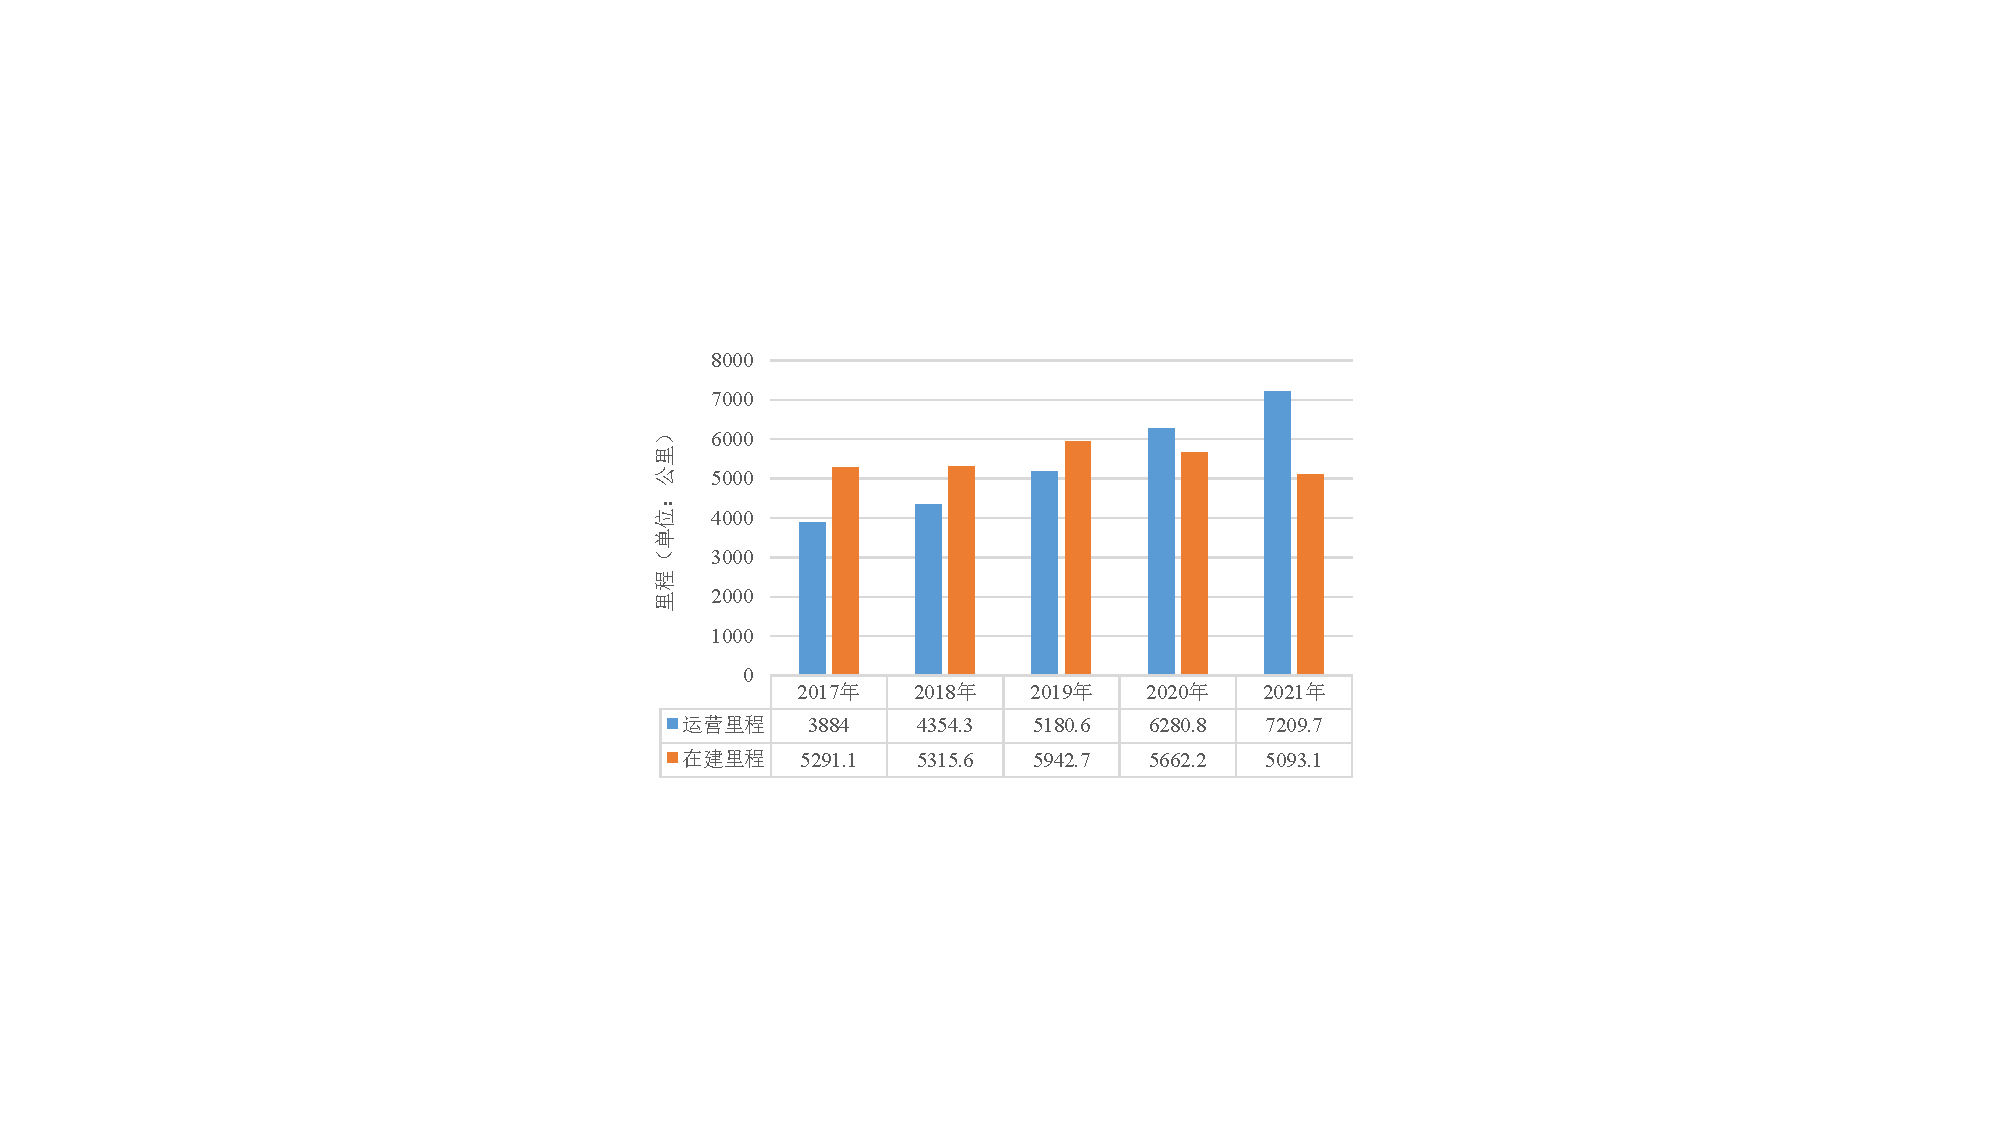
\includegraphics[width=8cm,height=4.79cm]{Fig/全国地铁在建里程和运营里程.pdf}
		\caption{\label{地铁运营里程和在建里程}近年地铁运营里程和在建里程}
	\end{minipage}%
	\begin{minipage}[c]{0.5\textwidth}
		\centering
		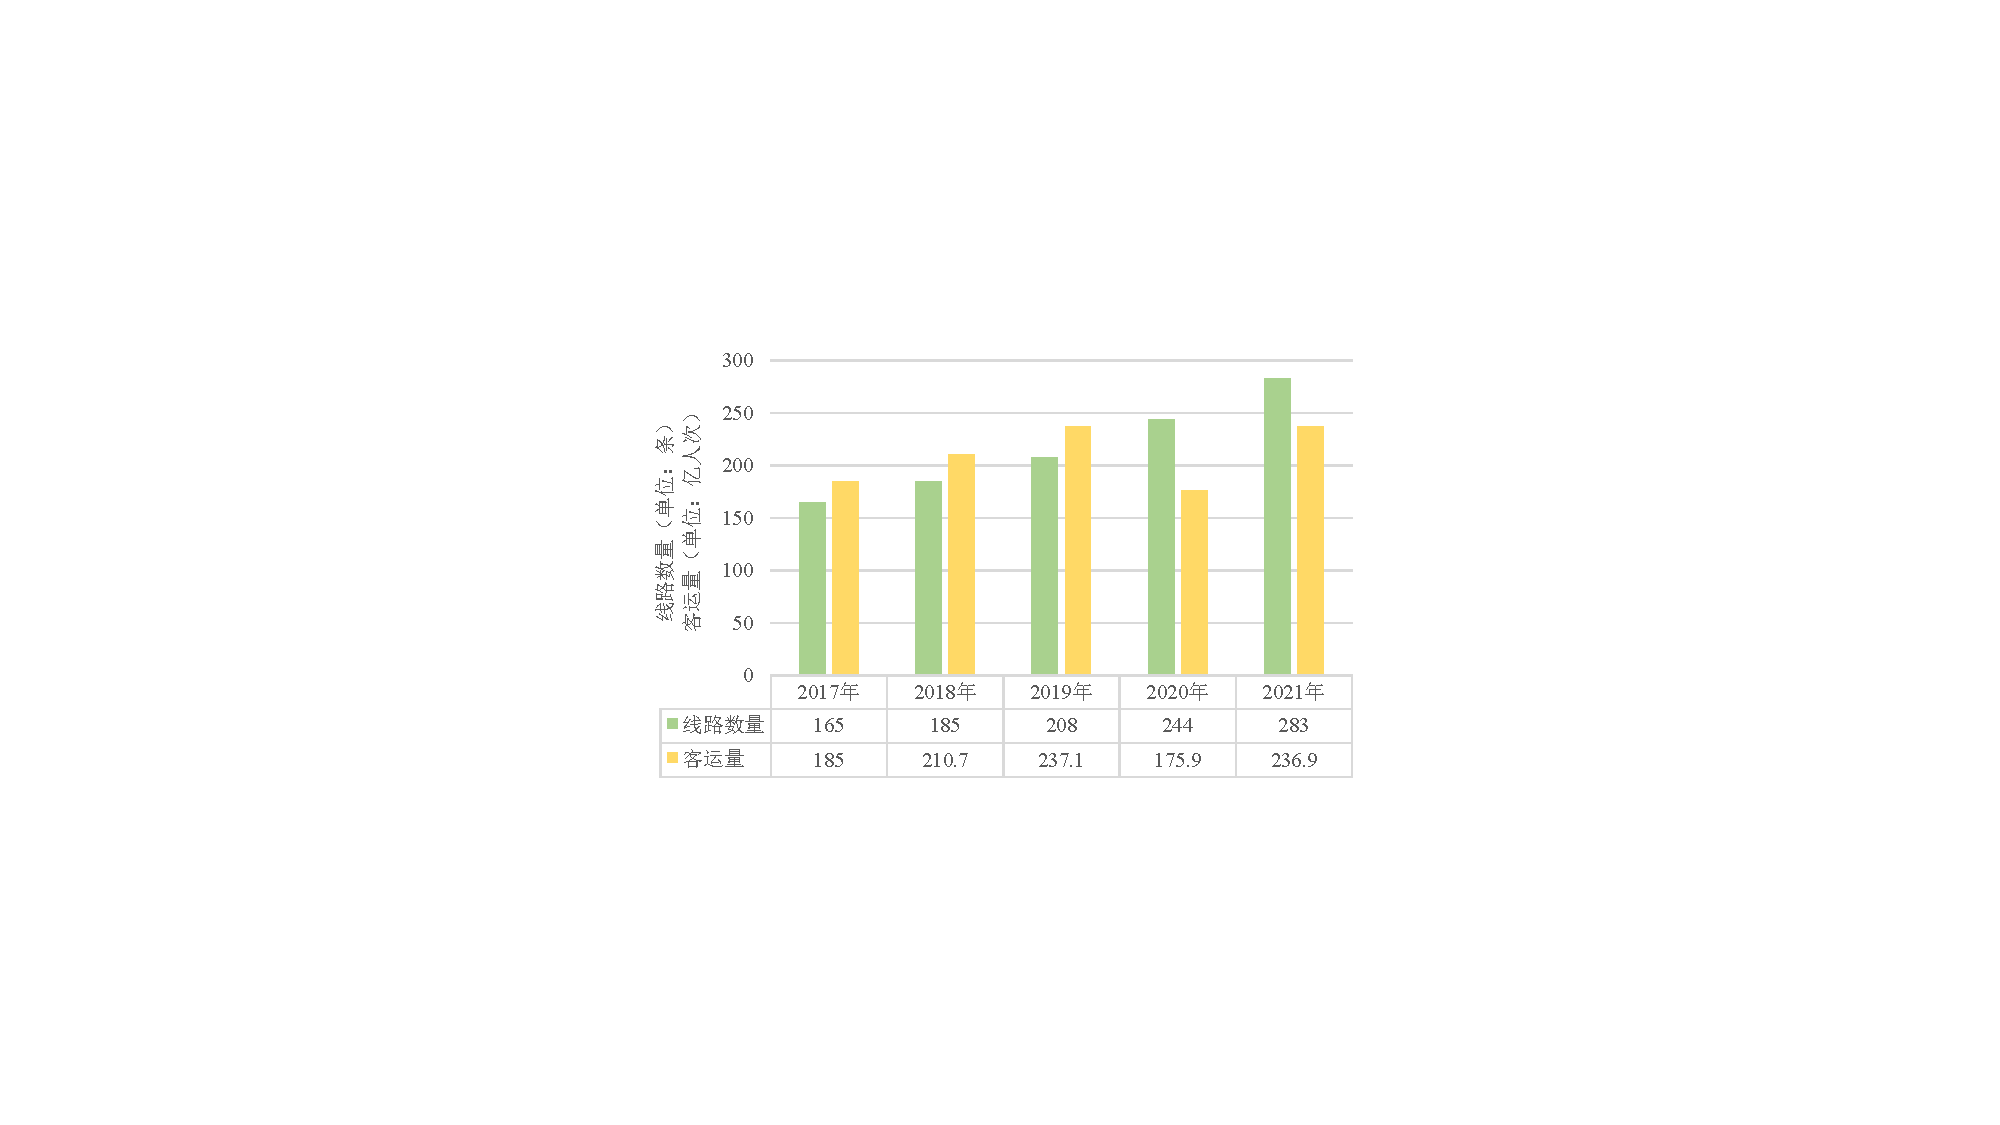
\includegraphics[width=8cm,height=4.79cm]{Fig/全国地铁运营线路数量和客运总量.pdf}
		\caption{\label{运营线路数和客运总量}近年地铁运营线路数和客运总量}
	\end{minipage}
\end{figure}

与地面交通相比,地铁运行受交通拥堵影响很小,且其自动化程度很高,能够有效地对列车实施直接的管理和控制,为乘客提供快速、准时、便捷的运输服务。为了出行方便,越来越多的市民选择地铁作为主要的出行方式,使得地铁客运量剧增。尤其在早晚高峰时段,车站的人流更是爆满,许多线路在早晚高峰时段列车最大满载率均超过100\%,部分区段高峰小时最达满载率超过120\%,相应的也产生了一些新的交通安全问题。为保障乘客的安全,地铁管理部门通常会在轨行区和站台候车区域之间安装屏蔽门(图\ref{屏蔽门}),将轨行区和站台候车区隔离。
\begin{figure}[htbp]
	\centering
	\subfloat[全高屏蔽门]{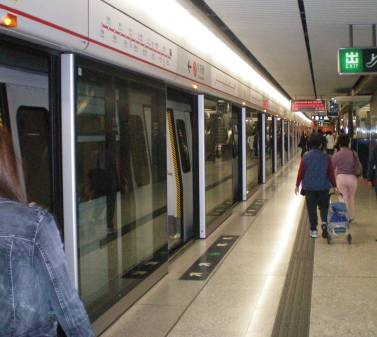
\includegraphics[width=6cm,height=6cm]{Fig/全高屏蔽门.jpg}%
		\label{全高屏蔽门}}\hspace{12mm}
	\subfloat[半高屏蔽门]{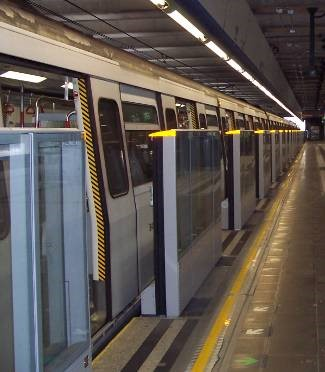
\includegraphics[width=6cm,height=6cm]{Fig/半高屏蔽门.jpg}
		\label{半高屏蔽门}}\hspace{12mm}
	\caption{屏蔽门}\label{屏蔽门}
\end{figure}

\begin{figure}[htbp]
	\centering
	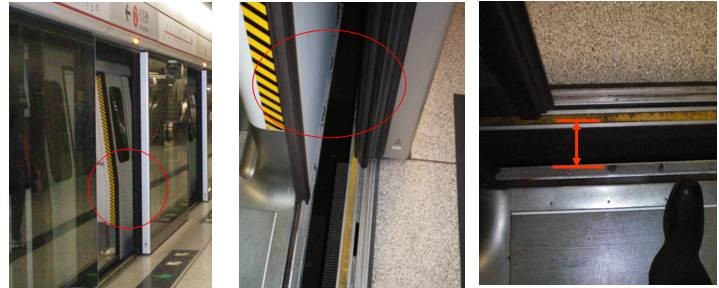
\includegraphics[scale=0.8]{Fig/屏蔽门缝隙.jpg}
	\caption{\label{屏蔽门缝隙}列车和屏蔽门之间存在一定宽度的缝隙}
\end{figure}
根据GB50157-2013《地铁设计规范》第5.3.8条\cite{地铁设计规范},车站直线地段建筑限界,应符合下列规定:车站设置站台门时,站台门的滑动门体至车辆轮廓线(未开门)之间的净距,当车辆采用塞拉门时,应采用 130 mm;当车辆采用内藏门或外挂门时,应采用 100 mm。但是由于城市轨道交通线路设计、站台施工及车辆的制造误差等多种原因,造成屏蔽门与列车车门之间的间隙(如图\ref{屏蔽门缝隙}所示)并非完全一致。而根据目前城市轨道交通站点普遍所采用的设施指标,屏蔽门和车门间存在 150~340 mm 不等的缝隙,以广州地铁 1 号~4 号线为例,屏蔽门与列车车门的空隙在 200~250 mm 之间\cite{陈铸昌2017屏蔽门与列车之间防夹装置应用分析及展望}。如果上下车时乘客过度拥挤,或有乘客在车门即将关闭时冲门,则可能会发生人或物被夹于空隙中的事故。而如列车启动前未能发现这些事故,依然正常驶出,那么可能将产生不良后果,严重时甚至会危及乘客的生命安全。

例如2014年11月6日,在北京地铁5号线惠新西街南口站,一名乘客在上车的时候被夹在地铁站台门与列车门的缝隙中间,因地铁工作人员未及时发现乘客被夹,列车继续运行导致该名乘客不幸身亡。2018年4月23日,在上海1号线宝安公路地铁站,一名女子被卡在地铁和屏蔽门中间,被地铁工作人员及时发现,打开屏蔽门得以脱身。2022年1月22日,在上海地铁15号线祁安路站,一位乘客下车时被屏蔽门夹住,但是列车仍然启动,导致该乘客不幸身亡。胡亚楠\cite{胡亚楠2017地铁屏蔽门、车门夹人成因分析及防范措施研究}更是对近年来广州地铁所发生的多起事故进行分析,发现屏蔽门与车门夹人造成安全事故的发生次数仅次于扶梯,占总受伤比例12.8\%。因此,消除地铁屏蔽门与列车门间夹人夹物这一安全隐患,是推动地铁高质量安全运行的必然要求,也是保障人民群众生命财产安全的现实需要。
\begin{figure}[b!]
	\centering
	\subfloat[无遮挡时灯带情形]{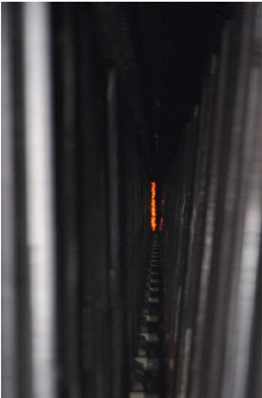
\includegraphics[width=5cm,height=6cm]{Fig/无遮挡时灯带情形.jpg}%
		\label{无遮挡时灯带情形}}\hspace{15mm}
	\subfloat[有遮挡时灯带情形]{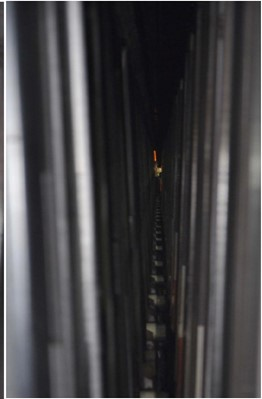
\includegraphics[width=5cm,height=6cm]{Fig/有遮挡时灯带情形.jpg}
		\label{有遮挡时灯带情形}}\hspace{15mm}
	\caption{列车尾部灯带的两种情况}\label{列车尾部灯带的两种情况}
\end{figure}

目前地铁屏蔽门与列车门间的异物检测主要依赖于人工瞭望:列车司机通过肉眼观察列车的尾部灯带是否被遮挡从而判断是否存在异物,如果被遮挡则说明有尺寸较大的异物存在于站台屏蔽门与列车门之间,具体如图\ref{列车尾部灯带的两种情况}所示。司机发现尾部灯带被遮挡后,还需要其他工作人员进行复检,确认是否存在异物并取出才能行车。然而随着客流量的日益剧增及地铁站台的样式各异,此种人工瞭望异物检测方法面临以下严重挑战:(1)受限于人眼视力,且地铁环境中光照亮度低,司机瞭望车尾灯带纵深距离远(120m-180m),判断灯带是否完整较困难,导致检测精度不高,检测盲区大,小异物的漏检率较高;(2)地铁站间距离通常只有几公里,且高峰期发车最短间隔低于120秒,在这短短时间内,司机需完成进站停车、开车门、人工核查、关车门、启动以及行驶等一系列操作,工作压力大,劳动强度高,极易疲劳,在此种状态人工判断将会存在较大的误检率;(3)人工瞭望方法仅能判断是否存在异物,而不能确定异物的位置及种类,还需站务人员在大概区间内逐一排查,效率较低。综上所述,通过人工瞭望的异物检测方式很难完全消除地铁屏蔽门与车门夹人夹物这一安全隐患,且效率不高。因此,亟需发展地铁屏蔽门与列车门间异物的智能识别检测技术,充分利用各种检测监测信息化技术,加强地铁站台、屏蔽门与列车门间、列车运行等的监控,实现地铁屏蔽门与列车门间异物检测应用系统的智能化升级,增强预警能力,加强过程控制,防范安全风险,保障地铁安全平稳运行,提升地铁运输业务的工作效率和经济效益。

近些年来,大数据、高算力、深度学习(Deep Learning, DL)、卷积神经网络(Convolutional Neural Network, CNN)等新兴词语映入人们眼帘,人工智能(Artificial Intelligent, AI)逐渐走向各类行业应用。2019年9月,国务院发布的《交通强国建设纲要》\cite{交通强国建设纲要}中指出,要大力发展智慧交通,推动大数据、人工智能等新技术与交通行业深度融合。2021年2月,在国务院发布的《国家综合立体交通网规划纲要》\cite{国家综合立体交通网规划纲要}中重点提到,要构建智能先进的现代化高质量国家综合立体交通网。2021年12月,国务院印发的《“十四五”现代综合交通运输体系发展规划》\cite{“十四五”现代综合交通运输体系发展规划}更是强调:推动互联网、大数据、人工智能、区块链等新技术与交通行业深度融合,推进先进技术装备应用,构建泛在互联、柔性协同、具有全球竞争力的智能交通系统。深度学习,凭借其自动提取特征、端到端学习等优势,在各个任务中取得了优秀的表现,是人工智能领域中当前最热门的架构。而随着地铁站中各处监测设备的大力部署,所获取包括图像数据在内的资源数据持续增长、各类深度学习算法的快速迭代更新以及国家政策的广泛支持,将大数据、深度学习等人工智能技术应用到地铁系统中以提升运输效率和安全也受到越来越多地关注。 

如图\ref{智慧地铁全生命周期}所示,人工智能及大数据等高新技术在地铁系统中的应用,可贯穿从最初的规划到最终的养护维修的整个智慧地铁全生命周期,应用前景十分广阔。人工智能参与智慧地铁全生命周期的具体研究方式主要包括将强化学习、视频智能分析、异常事件检测、目标检测、迁移学习等新方法、新技术应用于线路规划、监控预警、运营管理以及养护维修等场景中,实现真正的智慧地铁。本文将重点研究基于深度学习的目标检测算法在地铁屏蔽门与列车门间异物检测中的应用。
\begin{figure}[htbp]
	\centering
	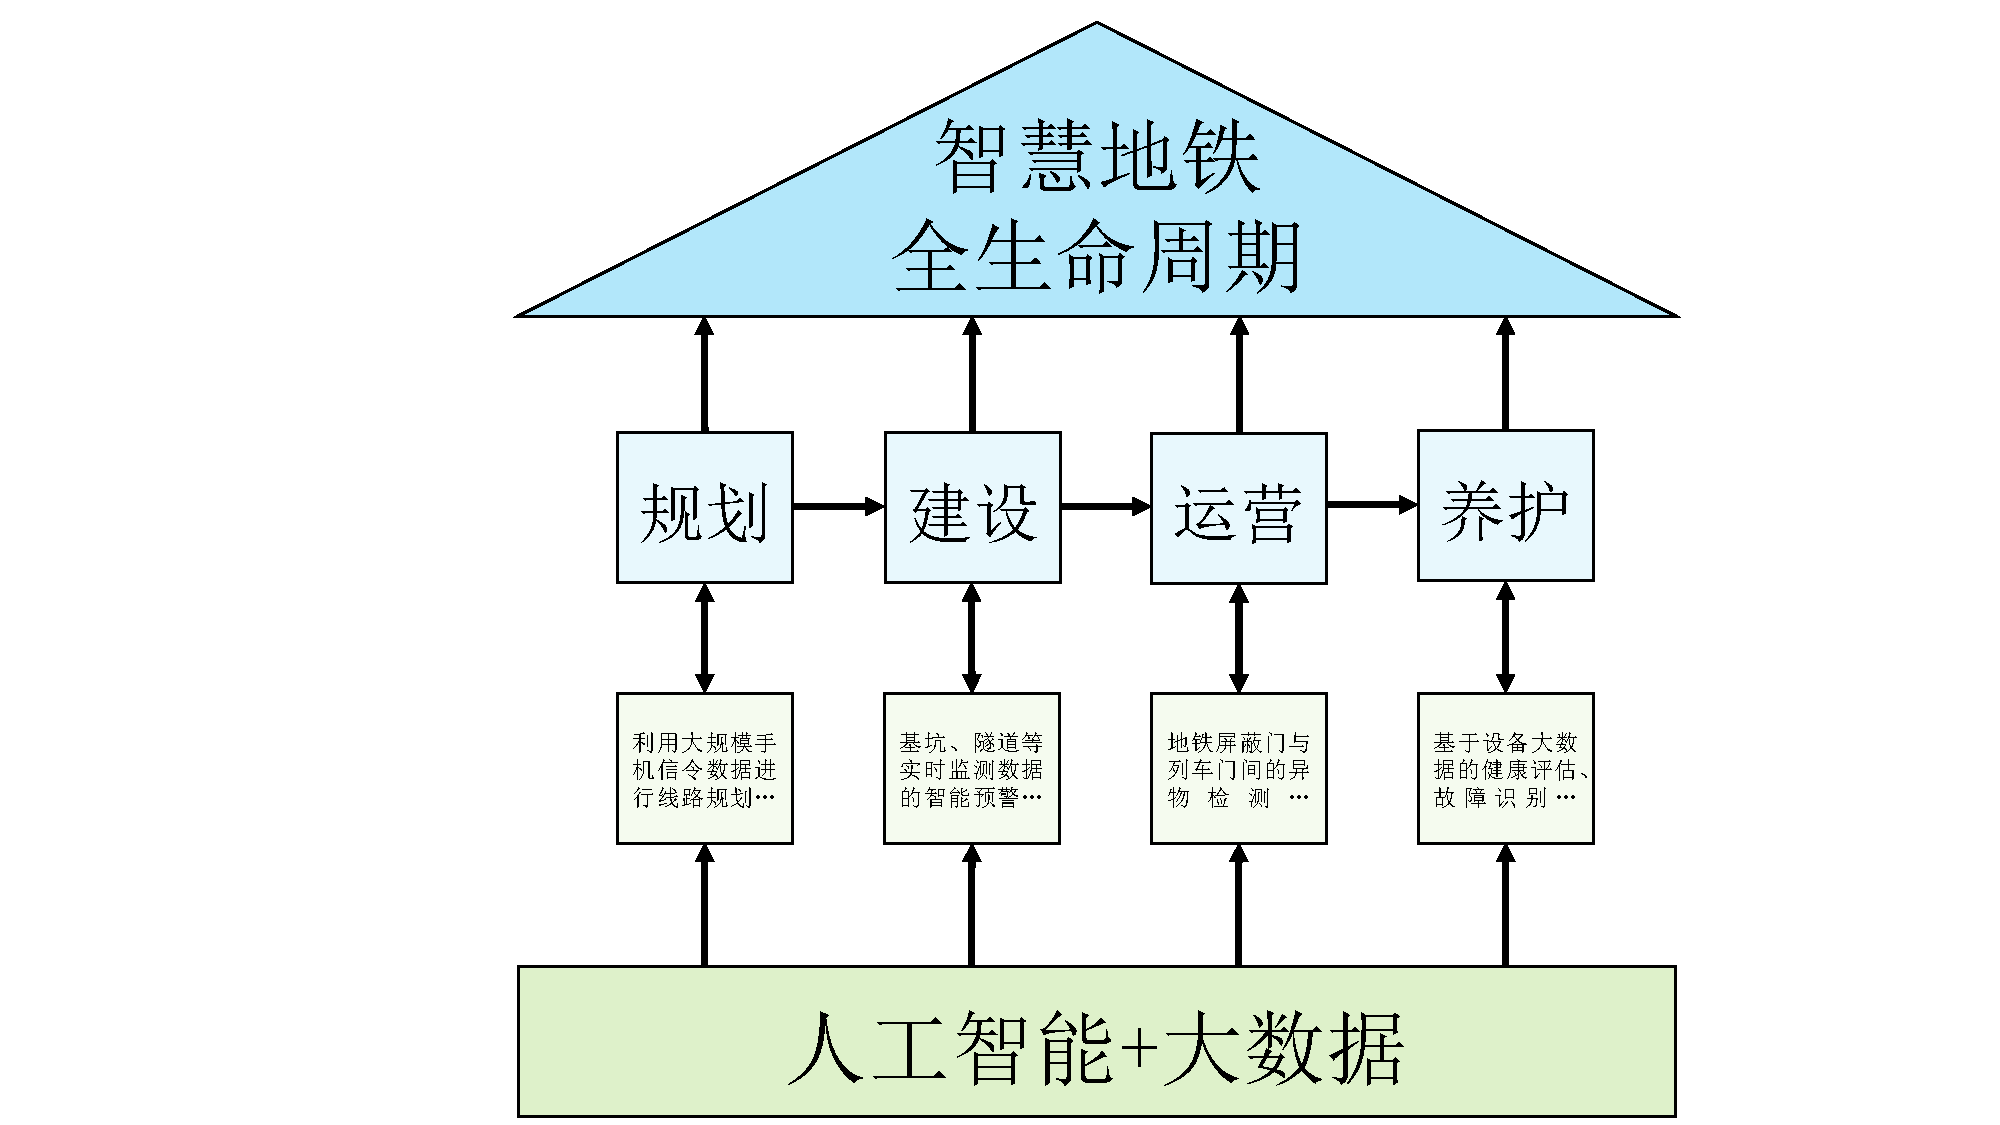
\includegraphics[scale=0.6]{Fig/智慧地铁全生命周期.pdf}
	\caption{\label{智慧地铁全生命周期}人工智能+大数据在智慧地铁中的应用}
\end{figure}

目前已有的对地铁屏蔽门与列车门间异物检测的研究主要集中在利用混合高斯背景建模(Gaussian Mixture Model, GMM)、Vibe算法等传统图像处理技术。一方面,这些传统图像处理技术很容易受到光照等外界环境的影响,鲁棒性不强,且检测精度不高;另一方面,前述传统图像处理技术只能简单地判断异物是否存在,而不能进行异物的识别。然而,异物种类的识别也是十分重要的:例如屏蔽门夹住乘客的身体,为最高风险等级,列车必须马上停止运行;而夹住的是衣角、布条,则可先保证运行效率再处理。基于深度学习的端到端目标检测算法在计算机视觉领域取得了突破性地进展,它首先能够自动提取特征,从图片数据出发,直接得到检测结果,并告知物体种类。因此,有必要研究基于深度学习的地铁屏蔽门与列车门间异物检测算法研究,采用先进的计算机视觉技术对屏蔽门与列车门间图像进行实时智能分析,检测异物,排除隐患,提高检测效率,保障生命和财产安全。站台屏蔽门与列车门是连接站台与列车的唯一通道,是地铁运输系统的风险点、瓶颈点和管控核心区域,直接影响地铁运输效率、安全等问题。屏蔽门与列车门间的异物检测是智慧地铁建设的重要研究内容。智能时代的到来,越来越多的全自动运行线路的开通,对异物检测提出了新的要求,也为其进一步发展提供了契机。因此应借力时代发展的快车,抓住新机遇,融合新理论,应用新方法,开创新技术,实现地铁运输全过程的高度信息化、自动化、智能化。 

鉴于此,本文在国家重点研发计划“城市轨道系统安全保障技术课题——运营环境区域内站台门与车门风险间隙乘客安全监测系统研制与示范”的支持下,以智慧地铁建设为背景,探索如何将深度学习、目标检测算法等更好地应用至地铁屏蔽门与列车门间异物检测领域,以期提高检测的准确性、实时性和有效性,进一步保障地铁的安全运行、保障乘客生命财产安全,提升运行效率。具体而言:一,本文将首先研究地铁屏蔽门与列车门间异物图像的半自动标注方法,解决以往大数据集标注所需大量人力资源问题;其次,从真实场景中收集数据,建立地铁屏蔽门与列车门间异物图像数据集,为异物检测算法建立统一性能测试平台。二,在所构建的异物图像数据集上研究地铁屏蔽门与列车门间异物检测算法,提高模型检测精度,满足辅助工作人员进行异物检测的要求;三,研究模型的轻量化,在尽可能小的降低模型检测精度的前提下,大幅降低模型的参数与计算量,满足低硬件条件下的实时检测要求;最后,根据现有地铁系统中图像监测系统的应用现状及其特点,研究适用于地铁屏蔽门与列车门间异物图像检测系统部署特点,基于全自动运行地铁系统线路总体架构,构建边云协同的地铁屏蔽门与列车门间异物图像智能识别平台,实现应用系统的智能化升级。
\subsection{研究意义}
地铁站台屏蔽门与列车门是连接站台与列车的唯一乘降通道,是地铁自动驾驶系统的风险区域、乘降瓶颈点和管控核心区域。实时精准的地铁屏蔽门与列车门间异物检测是构建智慧地铁生态的重要基础和核心任务,对保障地铁的安全运行及提升运营效率具有重要指导意义。只有在及时、准确地检测地铁屏蔽门与列车门间异物的基础上,才能更好地辅助控制中心工作人员进行地铁系统的管理与控制,进而实现全自动运行地铁系统的安全运营。

人工智能、深度学习等在计算机各类视觉任务中发挥了举足轻重的作用,相关的深度学习模型,凭借其良好的性能、鲁棒性强等优点,获得了巨大的关注,也逐渐深入到全自动运行地铁系统中的智能检测等领域,研究意义重大,主要分为以下几个方面:
\begin{enumerate}[topsep = 0 pt, itemsep= 0 pt, parsep=0pt, partopsep=0pt, leftmargin=44pt, itemindent=0pt, labelsep=6pt, label=(\arabic*)]
	\item 降低乘客安全风险。相比现有的人工瞭望等异物检测方式,本文所研究的异物智能检测技术可以大幅度提升夹人夹物等事件的检测准确率,有效消除地铁屏蔽门与列车门间夹人夹物的隐患,保证乘客在上下车时的生命安全,全面增加地铁运行的可靠性和安全性。
	
	\item 提升地铁运行效率。实时精准的异物检测系统无需再通过司机下车或工作人员现场走动对屏蔽门与列车门间的实际情况进行观测,减少了司机开关车门出入驾驶室的时间,进一步减少现有人工异物检测识别的消耗时间。通过对人工检测时间的优化,可以缩短每一趟列车的在站时间,从而提高列车的发车频率,增加列车的发车次数,保证列车的快速运行,大幅度的提升现有地铁系统的运输能力。
	
	\item 减轻人力资源消耗。异物检测系统可准确检测异物情况,自动识别并通过系统进行报警通知控制中心工作人员,控制中心工作人员可通过异物检测结果,根据具体情况及时进行指挥控制。通过异物系统的实时监测,可以减少地铁公司在列车运行过程中在站台区域配置的站务管理人员和屏蔽门报警维修人员数量1-2名,使整个管理部门更加合理有效地利用所有人员,合理分配人员的任务和工作。
\end{enumerate}
\section{国内外研究现状}
本节将首先给出本文所研究的地铁屏蔽门与列车门间异物检测的具体检测区域及所检测“异物”的定义;然后分析地铁系统的环境特点;在此基础上介绍当前地铁系统中各类异物检测系统的应用现状及基于深度学习的异物检测研究现状;最后基于研究现状调研结果总结既有应用系统及研究存在的不足。
\begin{figure}[b!]
	\centering
	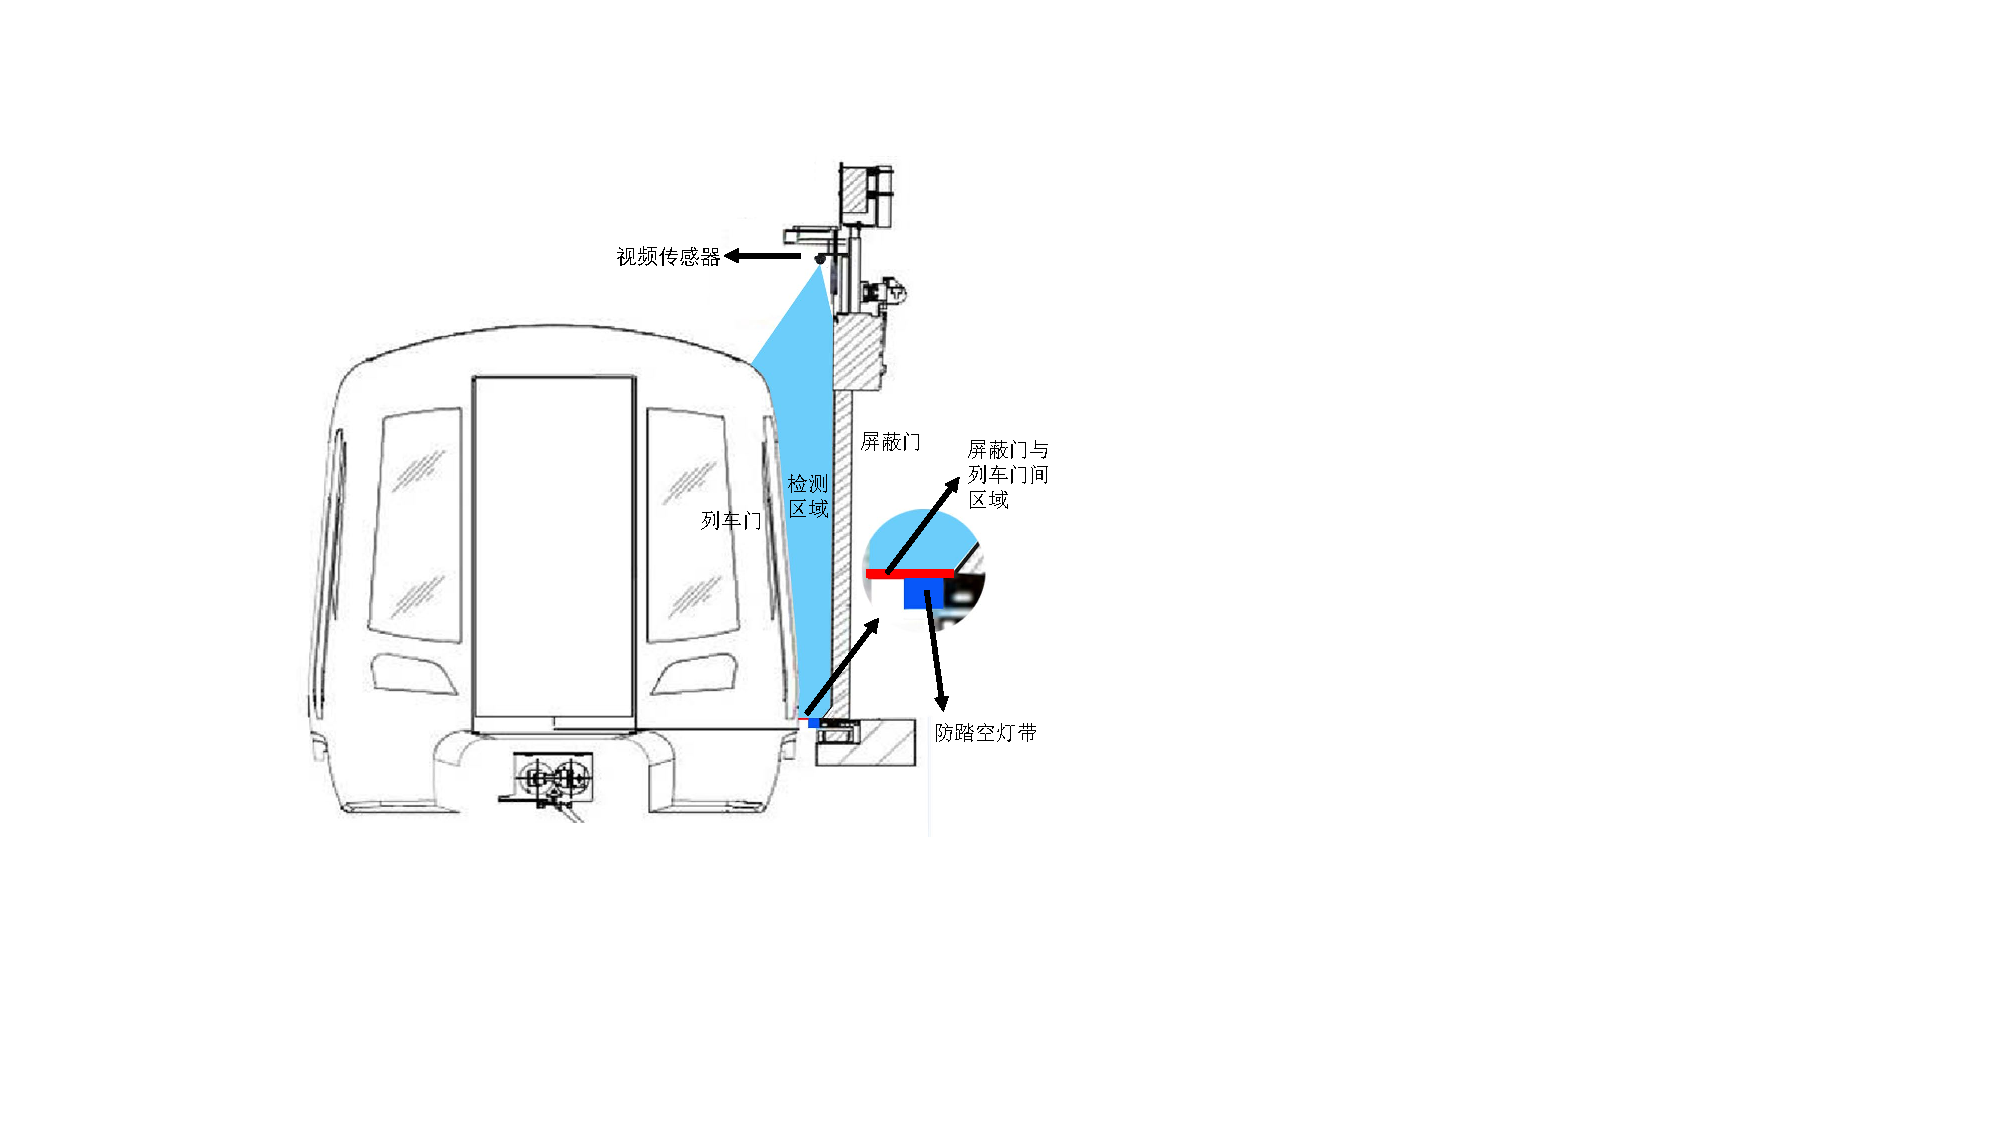
\includegraphics[scale=0.8]{Fig/检测区域.pdf}
	\caption{\label{检测区域}检测区域示意图}
\end{figure}
\subsection{检测区域及异物的定义}
\subsubsection*{检测区域的定义}
本文所研究的检测区域定义为屏蔽门门缝,列车门门缝以及两门间的立体区域(如图\ref{检测区域}所示)。检测区域的长度为整个地铁站台长度,一般为120米到180米。对于如此狭长的检测区域来说,仅通过人工瞭望很难排除掉所有安全隐患,因此亟需一种快速且精准的智能异物检测技术对屏蔽门与列车门间区域进行实时监测,辅助控制中心工作人员发现一些难以察觉的安全隐患。
\subsubsection*{异物的定义}
在列车与屏蔽门之间发生的安全事故主要是夹人夹物事件,这些事件主要包括列车与屏蔽门之间夹有行人;列车门缝夹有人,或者物;屏蔽门缝夹有人或者物品;屏蔽门踏板之上跌落下物品。常见被夹对象为人的手和脚,衣服,随身的包,以及女生的头发。常见的遗落的物品主要有雨伞,钱包,手机,水瓶等。因此本文定义空间异物为地铁屏蔽门和列车门关闭之后,列车驶离站之前;屏蔽门踏板以上,屏蔽门与列车之间空间新增的人或物品。
\subsection{地铁环境特点分析}
\subsubsection*{检测纵深长}
目前许多城市地铁列车采用6编组和8编组,站台长120~180米,异物检测纵深长(图\ref{地铁纵深长}),对检测设备要求高,需要能够对此狭长空间内的乘客或异物准确检测。
\begin{figure}[htbp]
	\centering
	\begin{minipage}[c]{0.5\textwidth} % minipage将页面划分为0.5\textwidth
		\centering
		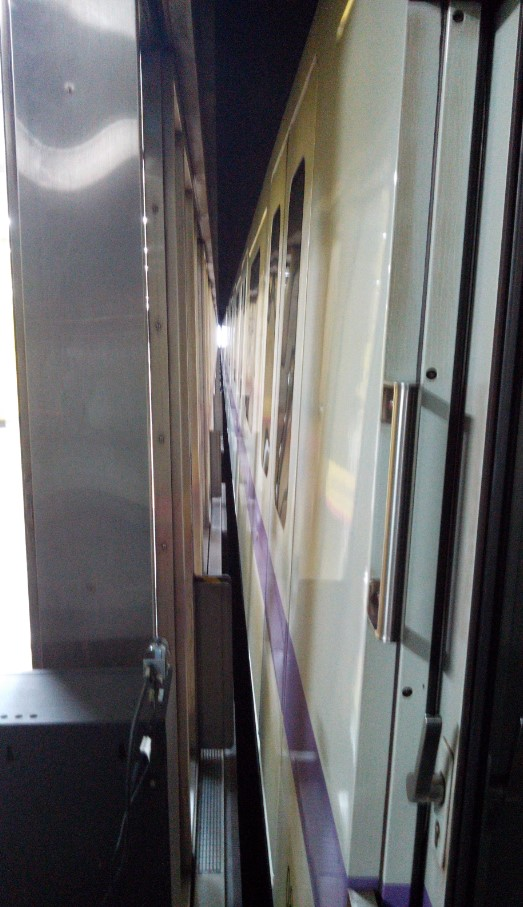
\includegraphics[width=6cm,height=8cm]{Fig/地铁纵深长.jpg}
		\caption{\label{地铁纵深长}地铁纵深长}
	\end{minipage}%
	\begin{minipage}[c]{0.5\textwidth}
		\centering
		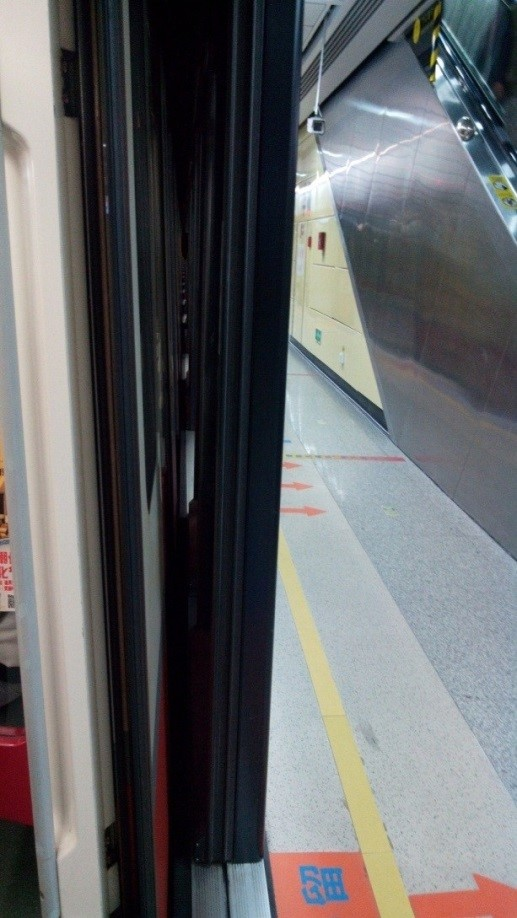
\includegraphics[width=6cm,height=8cm]{Fig/空间狭小.jpg}
		\caption{\label{空间狭小}空间狭小}
	\end{minipage}
\end{figure}
\subsubsection*{空间狭小}
地铁列车门与屏蔽门之间的空隙最小处只有约13厘米(图\ref{空间狭小}),可供安装设备的空间受限制,宽度仅有35mm。检测系统需要实现检测设备小型化,防止设备侵限。
\subsubsection*{环境干扰严重}
(1)震动:列车驶过使站台产生震动。(2)隧道风:列车驶过产生强烈的活塞风。(3)灰尘大:隧道风引起隧道内的粉尘,产生的悬浮粒子。震动、隧道风、灰尘大等特点易对检测结果造成影响,检测系统能够实现区域检测,达到对震动、隧道风等影响具有鲁棒性。
\subsubsection*{列车门多,异物存在位置不定}
根据列车编组不同,列车门有20~40个,异物可能存在于任何区间内,存在的位置、高度都不确定,且由于列车在站时间仅有20~40s,检测系统能够检测异物所处门号,从而能够快速清除异物,减少在站时间。
\subsubsection*{存在黑色异物}
列车门与屏蔽门风险间隙之间可能存在大量的黑色异物,黑色异物无法反射主动光,易造成漏检,需要检测设备采用自然光反射的视觉区域检测器。
\subsection{异物检测系统应用现状}
\subsubsection*{基于人工瞭望的异物检测}
广州地铁在2004年11月率先在全国研发并安装了屏蔽门站台瞭望灯带。目前,国内城市轨道交通系统几乎都是采用人工瞭望灯带进行检测,列车司机开车前先下车进行人工检查,通过肉眼观察地铁列车的车尾处的灯带是否完整,以间接判断是否有乘客被夹在列车与屏蔽门之间。地铁公司规定,列车启动前,司机(操纵者)必须确认关门灯、发车灯及发车音响信号显示状态,恢复门选项开关。确认出发信号机的进行显示(绿色灯光)并手指信号机,呼唤“换门良好,出站绿灯”缓解列车使用牵引一位启动,瞭望线路,开启头灯,观察仪表显示,待启动电流稳定后,逐位牵引,禁止直推牵引三位启动。瞭望台工作人员要扫视观察乘客是否全部上车,确认后抬手示意,列车司机进入驾驶室缓缓启动列车。若有乘客在站台上探出身子张望,行为危险,则大声呼喊或是广播提醒乘客,有必要时通过手台联系综控室。可见,这一系列的工作流程使得地铁司机与人工瞭望工作劳动强度大,且人工瞭望的准确性极易受地铁环境影响。
\subsubsection*{基于光电传感器的异物检测}
\subparagraph*{\textbf{红外光幕}}
红外光幕探测器技术利用接收端是否能接收到发送端输出的多束(3到6束)一般间距10cm的红外信号来判断是否有障碍物存在,成本较低。但由于光幕探测器发射信号的为红外光,光斑随着检测距离的增加逐渐增大,一对光幕探测器用于地铁障碍物检测的最大有效距离约为24米,光束间距最小不会大于10cm,故不适于远距离检测,一般采用多组接力方式实现屏蔽门列车门间异物检测;为防止因灰尘和悬浮粒与昆虫遮挡引起的误报,该检测方式一般要求同时遮挡3束光才报警,无法检测小物体,只能检测是否夹人,且由于表面十分光滑的车门和屏蔽门会折射/反射光,常会造成虚警或误报。一组光栅与另一组光栅易互相干扰,安装对位非常不容易,且安装后会遮挡屏蔽门端末的灯带。
\subparagraph*{\textbf{激光光幕}}
激光光幕检测器方式由激光发射器、激光检测器(接收器)或激光反射板组成,由一个或几个激光发射器向对应的激光接收器发射激光,如果接收端可以接收到发射激光则认为该区域畅通无障碍物,如果接收不到信号则认为发射激光被遮挡,则该区域存在障碍物。一般为2~3束间距大于25cm的激光。该检测方式中,激光较红外光聚光效果较好,有效检测距离较长,但由于激光光束易受到屏蔽门和列车车门材料属性所致均容易使发射的激光产生漫反射,导致在实际存在障碍物的情况下,发射信号容易绕过障碍物经列车或屏蔽门漫发射至接收器,使接收端仍能接收到发射端的信号,造成大量的误检,以及隧道灰尘、站台震动等,易引起虚警。因检测距离远,120到180米,该方式对准十分困难,对安装和抗震动要求极高。为防止因灰尘和悬浮粒与昆虫遮挡引起的误报,该检测方式一般要求同时遮挡3束光\cite{金仙力2020一种用于站台门障碍物探测的传感器系统及其探测方法}才报警,无法检测小物体,只能检测是否夹人。
\subparagraph*{\textbf{激光扫描}}
激光扫描仪主要由激光扫描发射器、激光扫描接收器等组成,利用飞行时间\cite{黄照东2021一种基于激光视觉的智能地铁站台屏蔽门异物探测器}(Time of Flight, TOF)原理扫描空间是否存在异物。激光扫描仪技术原理即发射器发出一个激光光线,打到物体表面后反射,再由接收器接收到反射回的光线,根据记录的时间差可测算距离。该检测方式为在每个或多个屏蔽门处安装一套激光扫描仪,根据扫描激光面数量的不同,有可分为单层激光扫描和多层激光扫描,单层激光扫描即扫描仪有1个激光扫描平面,多层激光扫描即扫描仪有多个激光扫描平面(一般为4个平面)。由于激光光束易受到屏蔽门和列车车门材料属性所致均容易使发射激光产生反射/折射,导致发射器发出的扫描光束无法返回接收器,从而导致漏检与误检,且仅能检测激光光幕扫描的平面内是否存在异物,无法将检测结果可视化。
\subsubsection*{基于视频传感器的异物检测}
\subparagraph*{\textbf{侧装视频传感器}}
侧装视觉传感器检测方案是一种安装成本低,维护简单的异物检测方案,并且应用场景较多,在半高站台门和无站台门情况下都可使用。刘伟铭\cite{刘伟铭2013直线地铁站台屏蔽门与列车间异物自动检测方法及其装置}发明了直线地铁站列车门和站台门异物自动检测方法及其装置专利。该专利主要是在列车尾部所在的站台处安装一个灯带,在列车头停靠方向的站台侧安装两个视觉传感器拍摄站台尾部的灯带,安装位置具体如图\ref{侧装视觉传感器}所示。将拍摄到的灯带图片利用图像处理技术得到清晰的灯带区域,通过判断灯带是否完整来进行异物检测。雷焕宇\cite{雷焕宇0基于机器视觉的户外站台列车和屏蔽门之间异物检测系统研究,雷焕宇2018基于}在车头部分利用视频传感器获得车尾灯带图像,然后利用K-Means 方法对所的图像进行目标提取,通过计算目标的完整性来检测异物。谭飞刚\cite{谭飞刚2017一种基于计算机视觉的地铁站台异物检测算法}提出检测方案与上述不同,将检测到的灯带与列车离站时保存的灯带模板图进行对比,如果灯带属性差异过大,则认为地铁风险区域内有异物。相比于人工瞭望灯带方式,该方案可以辅助地铁工作人员核验灯带是否完整,从而减少地铁工作人员的核查压力。但是上述侧装视觉传感器检测方案和人工瞭望灯带的缺陷是都只能对灯带所在的平面进行异物检测,有一定的检测盲区而且小尺寸异物很难被检测到。
\begin{figure}[htbp]
	\centering
	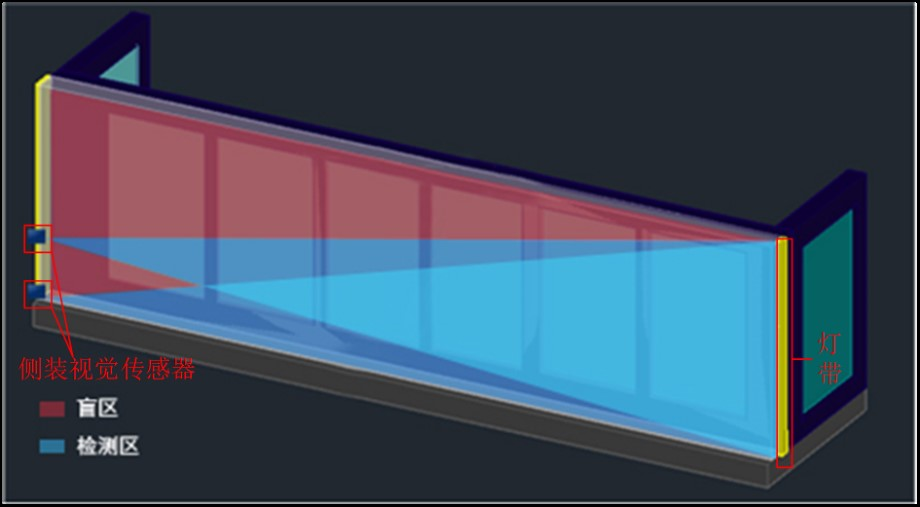
\includegraphics[scale=1]{Fig/侧装视觉传感器.jpg}
	\caption{\label{侧装视觉传感器}侧装视觉传感器和灯带安装位置示意图}
\end{figure}
\subparagraph*{\textbf{顶装视频传感器}}
顶装视觉传感器检测方案一般在每一个站台门的正上方安装一个视觉传感器,对采集的图像进行异物检测,具体位置如图1-25所示。该方案能够覆盖到地铁站台门与列车门间的全部风险区域,无检测盲区,而且可以反馈出存在异物的现场图像,辅助地铁工作人员发现人工检查过程中难以察觉的安全隐患。此外,因为在每个站台门上安装了视觉传感器,所以可以知道存在异物的具体车厢号和车门号,减少了盲目对每个车门进行复查所耗费的人力和时间,从而增强了地铁的运营效率。该方案还适用于曲线站台,完美地解决了工作人员因视线受阻而难以察看整个风险区域是否存在异物的问题。所以本文选择的检测方案为顶装视觉传感器检测方案,视觉传感器选择为彩色高清摄像头。
\begin{figure}[htbp]
	\centering
	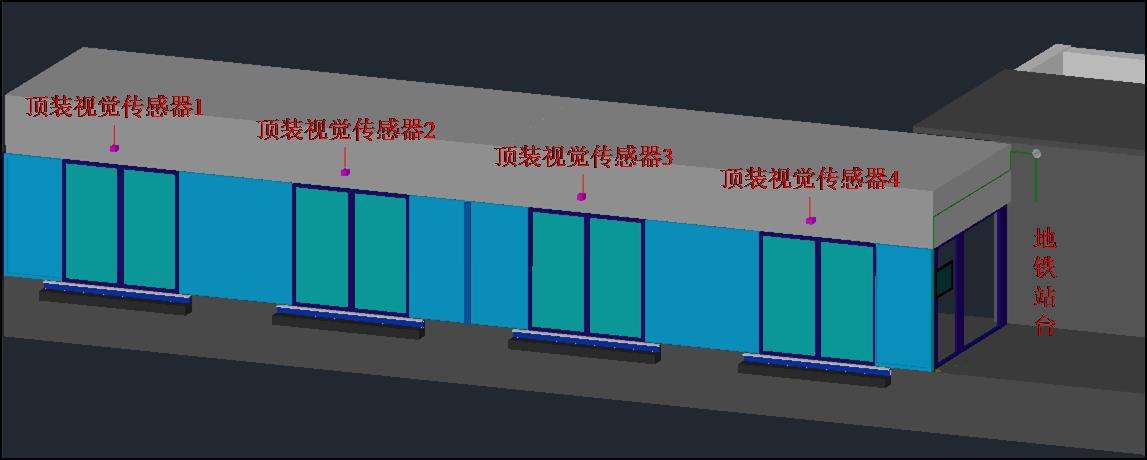
\includegraphics[scale=0.4]{Fig/顶装视觉传感器.jpg}
	\caption{\label{顶装视觉传感器}顶装视觉传感器安装位置示意图}
\end{figure}

对于顶装视觉传感器检测算法的研究,肖义\cite{肖义2019一种基于图像识别的站台门异物检测与报警的方法及系统}首先通过传感器获取预设范围内的无异物图像,然后根据预设背景类别对所得图像进行场景判别,最后将现场图像和预设背景图像进行比对,从而判断是否存在异物。同样的,谭飞刚\cite{谭飞刚2017基于机器视觉的地铁曲线型站台异物检测算法}先对无异物的图像进行混合高斯背景建模\cite{Improved-Adaptive-Gaussian-Mixture-Model-for-Background-Subtraction}(Gaussian Mixture Model, GMM),然后在与待检测图片进行差分,判断是否有异物。刘伟铭\cite{刘伟铭2021基于RGB-D}提出基于RGB-D和ViBe的前景检测算法,融合彩色和深度图像建立背景模型,然后再进行前景判断。上述基于传统图像处理的视觉传感器检测都容易受到光照等外界环境的影响,导致起决定性作用的超参数难以适应全部情况,要做到很高的检测精度比较困难。
\subsection{基于深度学习的异物检测研究现状}
由于地铁场景数据的保密性,目前应用在地铁站台门与列车门之间风险区域的异物检测方法不多。刘伟铭\cite{刘伟铭2021适用于地铁异物前景检测的神经网络——}提出的前景检测网络DifferentNet,通过解码器计算待检测图片和模板图之间的差异,得到前景热力图判断是否存在异物。虽然该方法能够实时进行异物检测,但是其依赖模板图进行差异对比。如果保存模板图之后光照等环境发生较大变化,检测效果会受到一定的影响。Liu\cite{RuikangLiu}提出基于生成对抗网络(Generative Adversarial Network, GAN)图像重建的无监督异物检测方法,根据检测图片和重建图片在特征空间和图像空间上的加权重建误差,构建异常分数特征图,利用特征差异确定异物位置。该方法只需要正常无异物的样本进行训练,定位精度(Area under curve, AUC)达到了96.4\%,但是其推断速度只有每帧0.72秒,而且该方法未进行异物分类。Dai\cite{Efficient-FOD}对将地铁屏蔽门与列车门间的异物检测视为一种特殊的目标检测,而对利用基于深度学习的目标检测算法进行地铁异物检测进行了探讨,实验结果证明使用基于深度学习的目标检测算法来解决地铁异物检测任务具有巨大潜力。Liu\cite{WeimingLiu-and-DedongHuang}提出多任务结构模型,将风险区域分割、区域线检测和异物检测的结果融合,进一步提升了异物检测精度。
\subsection{现状总结及存在的问题}
目前应用在地铁站台门与列车门间风险区域的异物检测方式主要有人工瞭望,基于光电传感器、视频传感器等检测方法。其中,在顶装视觉传感器检测的研究中,又分为使用传统图像处理技术及使用深度学习技术。总结现有研究情况,如下表\ref{现有研究情况对比}所示。
% Table generated by Excel2LaTeX from sheet 'Sheet1'
\begin{table}[htbp]
	\centering
	\caption{现有研究情况对比}
	\scalebox{0.85}{
	\begin{tabular}{cccccccc}
		\toprule[2pt]
		\multicolumn{3}{c}{检测方式} & 检测区域  & 检测精度  & 检测可视化 & 判断异物种类 & 可远程确认  \\
		\midrule
		\multicolumn{3}{c}{人工瞭望} & 盲区大   & 低     & 无     & 否     & 否   \\
		\midrule
		\multirow{3}[2]{*}{光电传感器} & \multicolumn{2}{c}{红外光幕} & 盲区大   & 低     & 无     & 否     & 否     \\
		& \multicolumn{2}{c}{激光光幕} & 盲区大   & 低     & 无     & 否     & 否     \\
		& \multicolumn{2}{c}{激光扫描} & 盲区大   & 低     & 无     & 否     & 否     \\
		\midrule
		\multirow{3}[4]{*}{视频传感器} & 侧装    & 传统算法  & 盲区小   & 较高    & 有     & 否     & 否    \\
		\cmidrule{2-8}          & \multirow{2}[2]{*}{顶装} & 传统算法  & 无盲区   & 高     & 有     & 否     & 是     \\
		&       & 深度学习  & \textbf{无盲区}   & \textbf{高}     & \textbf{有}     & \textbf{是}     & \textbf{是}     \\
		\bottomrule[2pt]
	\end{tabular}
}%
	\label{现有研究情况对比}%
\end{table}%

由表\ref{现有研究情况对比}可知,当前许多地铁系统中正在使用的基于光电传感器的检测设备都只能对设备所在的平面进行检测,检测盲区大而且容易误检和漏检,存在许多缺陷。基于视觉传感器的异物检测方案有侧装和顶装两种方式,各有优点和缺点。侧装视觉传感器检测方案应用场景较多,在半高站台门和无站台门情况下都可使用,安装成本低且维护简单,但是仍有部分检测盲区而且难以检测到小尺寸异物。顶装视觉传感器检测方案在安装多套视觉传感器后,能够对地铁的风险区域进行全方位地监测并反馈存在异物的具体车门号以及现场画面。随着全自动运行地铁的蓬勃发展,顶装视觉传感器检测方案因其检测无盲区且可以将检测结果可视化等优点成为目前辅助地铁工作人员进行异物检测的发展趋势,本文的研究也正是基于顶装视觉传感器检测方案所进行。

基于顶装视觉传感器的异物检测算法主要分为传统图像处理算法和深度学习方法。传统图像处理算法因为存在大量的超参数难以适应光照干扰等环境变化,异物检测效果不稳定。此外,传统图像处理算法使用SVM等方法进行异物分类时候,模型本身的表达能力不强,从而导致分类的准确率不高。然而,告知工作人员异物的种类在地铁运营中是非常重要的。如果在地铁列车门和站台门两者间的缝隙遗留手机等电子产品,随着列车启动带来震动,该异物极有可能会掉落到轨行区中。如果能及时发现异物是手机这种电子产品,可以马上通知地铁工作人员停车并携带工具将手机取出,避免列车碾压手机产生火花从而造成重大交通事故。近年来,基于深度学习的目标检测方法由于不需要对图像进行复杂的预处理,且具有更强的模型表达能力,能够取得优秀的端到端目标检测结果。然而,目前基于深度学习的目标检测算法仍存在以下缺陷:(1)深度学习模型往往需要大量的数据才能得到充分的训练;(2)当前基于深度学习的目标检测算法通常基于卷积神经网络架构或者是近来兴起的Transformer架构,这两种架构各有优点,卷积神经网络擅长于局部特征的提取,而Transformer则在捕捉长距离依赖关系方面具有优势;(3)现有的深度学习往往运行于高性能计算平台上,而在实际工程中,并不是所有的硬件都能支持深度学习的训练。

综上所述,研究地铁屏蔽门与列车门间异物检测急需解决以下问题:
\begin{enumerate}[topsep = 0 pt, itemsep= 0 pt, parsep=0pt, partopsep=0pt, leftmargin=44pt, itemindent=0pt, labelsep=6pt, label=(\arabic*)]
	\item 现有的人工瞭望,光电传感器等检测方法存在诸如盲区大、检测精度低等缺点,并不能满足全自动运行系统所需异物检测系统的要求。因此需要研究在顶装视觉传感器方案下,基于深度学习的目标检测算法,能够无盲区、高精度的实现异物检测,并做到检测结果可视化、远程确认并判断异物类别。
	
	\item 建立统一、规范的数据集。因此需要构建
	
	\item 目前基于深度学习的目标检测算法往往依赖于某一种架构,缺乏将局部特征和全局特征相结合的能力。因此需要研究结合当前CNN和Transformer架构的优点,打造充分利用特征信息的目标检测算法。 
	
	\item 当前的基于深度学习的目标检测算法往往依赖于高性能计算平台的支撑,而在地铁环境中,能够分配给异物检测的硬件资源往往有限。因此需要研究深度学习模型的轻量化,使得模型能够在较低算力的前提下取得较好的效果。此外,还需结合边缘计算、云边协同等新技术,最终实现智能识别系统。  
\end{enumerate}

总体而言,在数据规模越来越大和信息越来越丰富的时代,在硬件设备不断更新和深度学习技术越来越普及的大技术背景下,地铁智能监控已经逐渐进入AI时代,深度神经网络的轻量化算法研究是本论文的核心研究任务。
\section{论文研究目标与内容}
地铁屏蔽门与列车门间异物检测涉及许多技术理论,本文的研究重点是利用基于深度学习的目标检测算法在全自动运行地铁系统中安全图像检测监测系统中的关键技术研究及总体应用架构。继承和借鉴计算机视觉中目标检测方面的成果,充分利用地铁站点中已存在的信息基础设施资源,以实现全自动运行地铁系统中安全图像检测监测系统智能化升级的可持续发展为目标,以地铁屏蔽门与列车门间异物检测的实际需求为出发点,从全局的视角提出基于深度学习的地铁屏蔽门与列车门间异物检测应用总体架构,构建云边协同的图像智能检测平台,为图像视频数据的统一管理和综合分析提供基础,为图像智能识别在全自动运行安全检测监测应用系统的推广使用起到指导性作用。 
围绕以上总体目标,本文主要以地铁屏蔽门与列车门间图像为研究对象,以深度学习算法为研究核心,结合全自动运行地铁中图像检测监测应用系统的特点,研究目标检测、模型压缩、边缘计算等先进信息技术在全自动运行地铁图像智能识别中的应用。主要研究内容如下: 
\begin{enumerate}[topsep = 0 pt, itemsep= 0 pt, parsep=0pt, partopsep=0pt, leftmargin=44pt, itemindent=0pt, labelsep=6pt, label=(\arabic*)]
	\item \textbf{数据集构建及图像半自动标注方法研究}:针对高速铁路运行安全图像由于缺乏大量带标注的数据集而阻碍了深度学习技术在高铁安全运行业务领域的成功及深入应用,且手工标注数据费时费力,研究高速铁路运行安全图像半自动标注方法,应用深度主动半监督学习的机器学习方法,充分利用已标注的数据,挖掘无标注数据资源的有用信息,最大化高铁运行安全图像智能识别应用的性能,而良好的图像标注技术对于图像的存储、管理以及数据集的建立及使用有很大的益处。
	
	
	\item \textbf{基于卷积神经网络和Transformer的异物检测方法研究}:针对动车组运行安全图像缺陷检测精度低的问题,研究应用基于深度卷积神经网络的目标检测算法解决动车组运行安全图像缺陷检测的实际问题,分析动车组运行安全图像及其缺陷形态的特征,优化基于卷积神经网络的目标检测模型,同时克服了复杂背景下正负样本不平衡和缺陷形态尺寸变化多样的困难,提高动车组运行安全图像缺陷检测的精度。
	
	
	\item \textbf{基于高效网络结构设计和模型压缩的轻量化网络研究及实际部署}:针对高铁接触网悬挂运行状态监测图像中小目标紧固件缺陷检测问题,研究应用基于深度学习的方法来解决高铁接触网运行状态监测图像缺陷检测的实际问题,深入分析监测图像的特点,对比接触网悬挂紧固件缺陷检测与自然图像目标检测的不同,将紧固件缺陷检测问题转换为紧固件检测和缺陷识别两个过程,提出基于两阶级联轻量级卷积神经网络的紧固件缺陷识别方法。 
	
	\item \textbf{全自动运行系统地铁屏蔽门与列车门间安全图像智能识别应用总体架构研究}:针对路网中高速铁路运行安全图像检测监测信息系统的应用现状及其特点,采用大数据、云计算、人工智能、机器学习、深度学习、边缘计算等先进的信息技术,充分高效利用铁路网中已有的信息基础设施,研究高速铁路运行安全图像智能识别应用总体架构,高铁运行安全图像智能识别平台的逻辑架构和功能架构,为高铁运行安全图像检测监测系统智能化升级提供基础支撑。  
\end{enumerate}
\section{论文的章节安排及组织结构}
\subsection{章节安排}
本文的具体章节安排如下:
第一章 绪论部分,介绍了课题的研究背景、研究意义、技术难点,简要介绍了铁路维护中基于机器视觉的高速铁路机械零部件无损检测的研究现状。动车组目标序列图像与对应的参考序列图像配准与对齐过程中求解相机位姿的P3P问题。最后简要介绍了论文的研究目标、内容,并给出了论文的章节安排。
 
第二章 目标检测相关理论。

第三章 数据集构建及半自动标注工具的设计。针对动车组裙板螺栓缺失的问题,提出了一种基于图像对齐与背景差分法的视觉检测模型。目标图像与参考图像的精确对齐是动车组裙板螺栓缺失检测的关键。根据目标图像与对应参考图像之间的水平偏移和垂直偏移对目标图像进行校正,实现裙板螺栓感兴趣区域(ROI)的精确对齐。本章提出了一种背景差分法用于定位缺失的裙板螺栓。最终,根据先验知识确定可能缺失的裙板螺栓,并通过使用高级图像理解知识来确定裙板螺栓的工作状态。

第四章 鉴于动车组列车底部异常位置的不确定性,动车组列车底部的异常检测需以动车组列车底部的序列图像为研究对象。GESIFT在提取关键点时进行了两次梯度的计算,确保了裙板序列图像感兴趣区域内关键点提取的鲁棒性,但在提取动车组列车底部序列图像的关键点时,计算效率较低。针对该问题,对基于GESIFT的图像对齐模型进行了改进,大幅度提高了动车组列车底部序列图像的对齐效率。在对动车组列车底部异常定位时,改进了背景差分模型,进一步增强了异常区域的特征,同时削弱了背景差异对定位结果的影响。

第五章 在SSD模型的基础上引入新的特征融合和注意力机制,以此对动车组底部出现的螺钉缺失、布条和纸屑等异常情况进行检测。新的特征融合策略有效利用了SSD模型浅层的细节信息和深层的语义信息,提高了SSD模型的平均检测精度,尤其是对小尺度异常目标的检测精度。注意力机制有助于在特征图的空间建立特征之间的关系,通过对全局相关信息的利用,突出有用信息,抑制不相关信息,为动车组列车底部的异常检测提供了可靠的指导。

最后,总结了本文的主要研究内容和创新之处,分析了本文研究的不足之处,展望了未来的研究方向,阐述了下一步工作计划,并对未来技术的运用做了适当的展望。
\subsection{组织结构}
本文的组织结构如下图所示:
\begin{figure}[htbp]
	\centering
	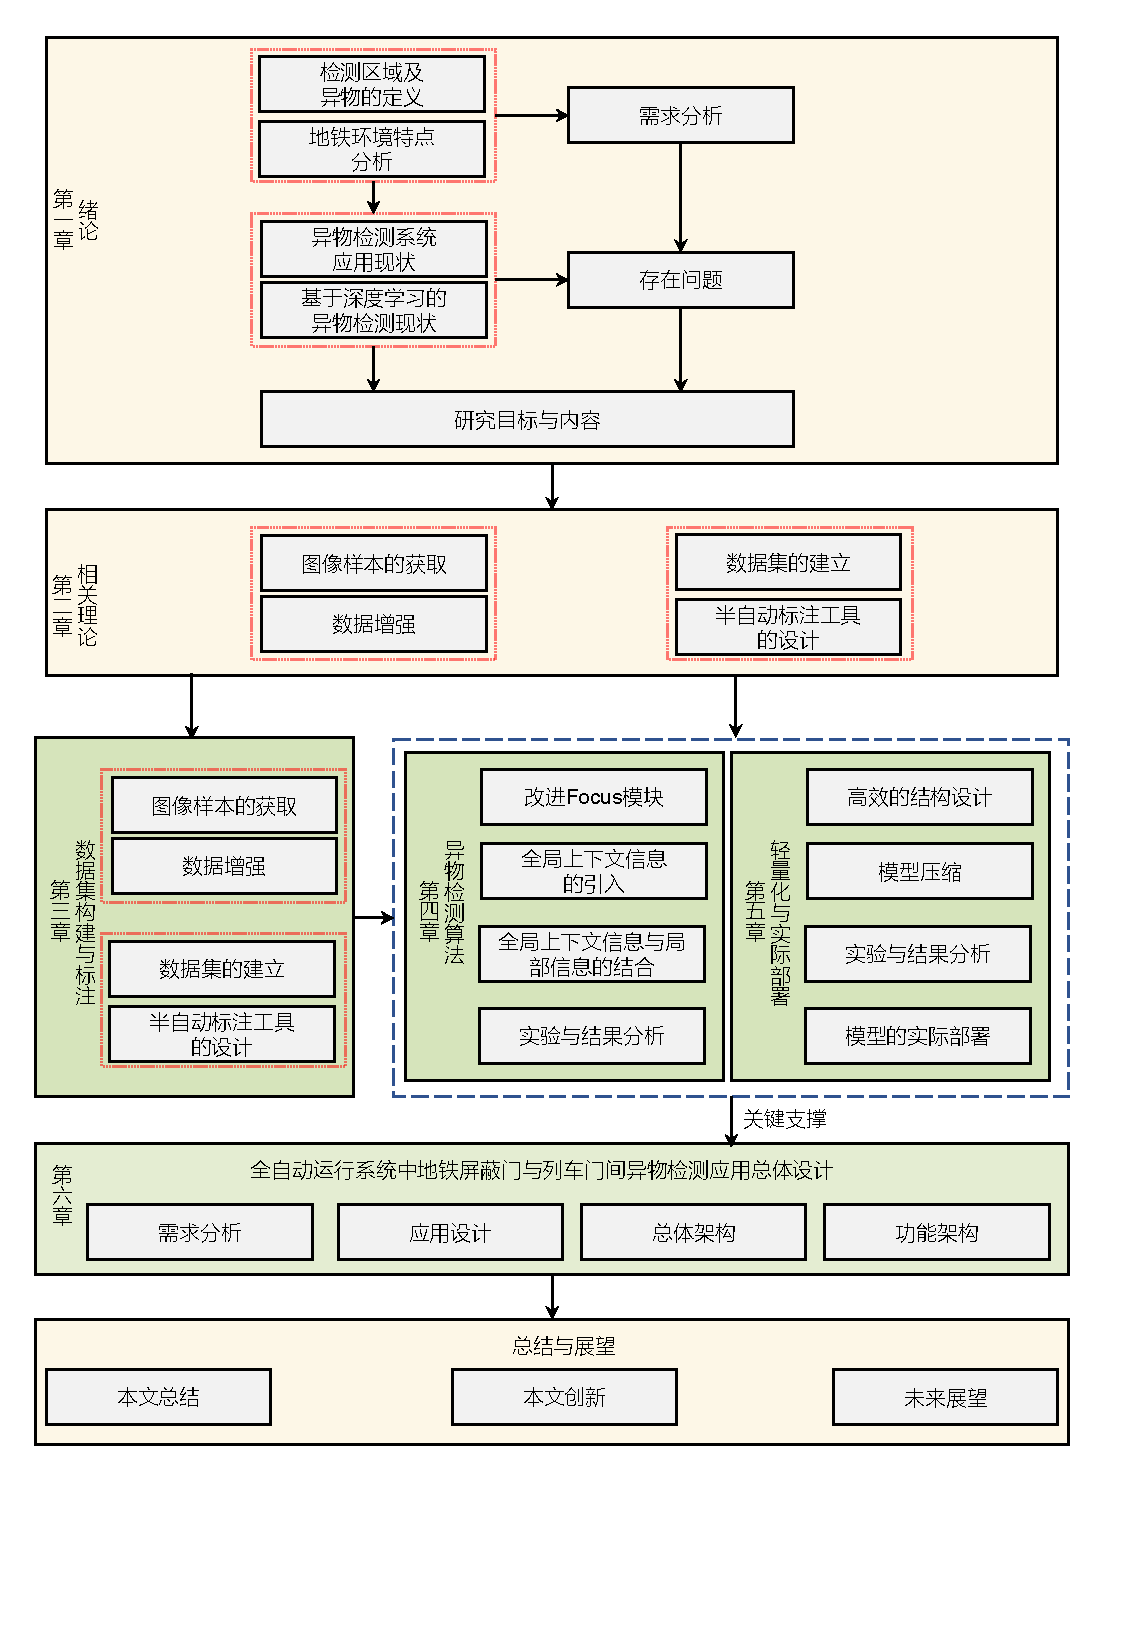
\includegraphics[scale=0.8]{Fig/文章框架.pdf}
	\caption{\label{论文的组织结构}论文的组织结构}
\end{figure}%第一章
	\chapter{相关基础理论方法}
\section{引言}
\section{基于深度学习的目标检测}
\subsection{基于卷积神经网络的目标检测}
\subsection{基于Transformer的目标检测}
\section{模型轻量化}
\subsection{高效的网络设计}
\subsection{模型剪枝}
\section{边缘计算}
\section{本章小结}

%第二章
	
\chapter{异物检测数据集的构建及半自动标注}
强烈建议在使用公式、表格、定理环境时进行百度,没必要研究各种用法,只需要知道自己需要什么。因本人的论文所用表格较少,因而对表格不是很熟悉,本章对表格的介绍相应的较少。本章仅介绍本人在论文撰写过程中常用的环境以及参考文献设置。

\section{引言}
\section{问题分析}
\section{异物检测数据集的构建}
\subsection{图像样本的获取}
\subsection{数据增强}
\subsection{数据集的基准格式}
\section{半自动标注工具的设计}
\section{本章小结}
%第三章
	\chapter{全局上下文信息与局部信息相结合的异物检测方法}
第三章主要针对地铁屏蔽门与列车门间异物检测应用中首先需要解决的数据集构建及数据标注问题进行了探讨和研究。本章在具有标注数据的前提下,主要研究应用基于深度神经网络的目标检测算法解决地铁屏蔽门与列车门间异物检测的实际问题,分析地铁屏蔽门与列车门间异物图像特征,优化基于聚类算法的锚框生成,同时克服了复杂背景下全局信息利用不足的困难,将其同局部信息有效的结合,提高地铁屏蔽门与列车门间异物检测的精度。

\section{引言}
我国地铁行业高速发展,运营线路、运营线路总长度、客运量等均居世界前列。为了出行方便,越来越多的市民选择地铁作为主要的出行方式,造成客运量越来越大。尤其在早晚高峰时段,车站的人流更是爆满,许多线路在早晚高峰时段列车最大满载率均超过100\%,部分区段高峰小时最达满载率超过120\%,相应的也产生了一些新的交通安全问题。而地铁屏蔽门与列车门间又是连接站台与列车的唯一乘降通道,是地铁系统的风险空间、乘降瓶颈点和管控核心区域。在地铁屏蔽门与列车门间出现异物,即使是细小的手机、雨伞等遗留物,也可能造成灾难性事故,及时发现异物并判断异物类别,可以提升地铁的运输效率和安全保障。在过去,地铁公司大多使用人工瞭望进行检测。然而,人工瞭望这一工作劳动强度大,且准确性易受地铁环境影响,并不能满足地铁系统要求。后来,地铁公司使用红外光幕、激光光幕、激光扫描等光电传感器来进行异物检测。但是,这些光电传感器仍然存在成本高、盲区大、检测效果不理想等缺陷,同样不能很好地满足需求。近年来,随着视频传感器设备及图像处理技术的发展,一些学者开始研究将计算机和图像处理技术应用于地铁屏蔽门与列车门间的异物检测。当前存在两种形式的视频检测系统:侧装式及顶装式。在检测盲区方面,侧装式系统仍然会存在一定的盲区。而在检测算法方面,侧装式及一部分顶装式检测系统中仍采用背景建模及模板匹配等传统图像处理算法,需人工设计特征且鲁棒性不强,极易受到外界环境影响,且不能自动判断出异物类别,需工作人员进行二次识别,效率低下。因此,使用顶装式检测系统,并改进地铁屏蔽门与列车门间异物检测系统的图像识别算法,提高异物检测精度,实现异物的自动检测具有重要的意义。

\section{问题分析}
地铁屏蔽门与列车门间是连接站台与列车的唯一乘降通道,情况复杂,人员众多,在两门开启关闭过程中,容易出现异物遗留的情况,如手机、雨伞、钱包,乘客等,若不及时发现及处理异物,将会影响地铁列车的正常工作,导致乘客人身安全及地铁运行安全受到威胁。据统计\cite{刘伟铭2019地铁风险空间分析及异物检测系统技术要求},某城市地铁站在2017年发生造成延误的异物事件共101起,各事件的比例按从大到小排列,如图\ref{异物事件比例}所示:(1)大部分异物事件为雨伞、水瓶、钱包等小异物体遗落站台边缘,占比 35.87\%;(2)由于客流拥挤,列车门启动防夹功能事件,占比 16.30\%;(3)列车门与屏蔽门夹乘客手指、手臂、头发等事件,占比16.30\%;(4)乘客背包包带被夹事件,占比14.13\%;(5)乘客衣服被夹事件,占比9.78\%;(6)最后,其他微小异物(如瓶盖、金属徽章、佛珠等)遗留事件,占比 7.61\%。
\begin{figure}[htbp]
	\centering
	
\includegraphics[scale=1]{Fig/异物比例.pdf}
	\caption{\label{异物事件比例}地铁屏蔽门与列车门间异物事件比例}
\end{figure}

本章以地铁屏蔽门与列车门间异物检测为主要研究任务,该任务存在两个主要的特点:
\begin{enumerate}[topsep = 0 pt, itemsep= 0 pt, parsep=0pt, partopsep=0pt, leftmargin=44pt, itemindent=0pt, labelsep=6pt, label=(\arabic*)]
	\item 现有基于锚框的深度学习目标检测算法在锚框生成这一步骤中,通常存在两种生成方法,手工方法和聚类方法:手工方法即为手工挑选锚框的尺寸,而聚类方法则通常是使用K-means 聚类算法自动找到良好的锚框。然而,这两种方法均存在一定的缺陷:手工方法需要人工挑选,工作强度较大,网络虽然可以通过学习适当地调整锚框形状,但是如果从一开始就为网络选择更好的锚框,就可以让网络更容易学习并获得更好的检测结果。而使用K-means聚类算法来生成锚框则受限于K-means 聚类算法本身的局限性,聚类结果很容易受到初始值的选取影响。因此,如何更好地自动生成锚框是第一个挑战。
	
	\item 以VGGNet\cite{vggnet}、InceptionNet系列\cite{Inceptionv1,Inceptionv2,Inceptionv4}和 ResNet系列\cite{resnetv1,resnetv2,resnetv3}为代表的卷积神经网络 (ConvNets)在多种视觉任务中取得了巨大的进展,它们的共同特点是顺序堆叠多个基本模块,并采用金字塔结构,但是却忽略了显式建模全局上下文信息的重要性。自从 2020 年以来,视觉 Transformer\cite{ViT,detr,Deformable-detr}进一步促进了视觉识别模型的发展,在ImageNet图像分类和下游任务上表现出比最先进的ConvNets更好的结果。这是因为与只进行局部建模的卷积操作相比,Transformer中的自注意力机制能够对全局的成对依赖进行建模,提供了一种更有效的空间信息编码方法。然而,在处理高分辨率图像时,自注意力机制导致的计算成本是相当大的。同时,许多研究\cite{Inside-OutsideNet,Combining-Multiple-Sensors-for-Event-Detection-of-Older-People,Attentive-Contexts-for-Object-Detection}已经证实,全局上下文信息可以为目标检测带来性能提升。在地铁这一复杂巨系统中,全局上下文信息对于异物检测同样也是至关重要的。因此,如何将Transformer擅于捕捉长距离依赖关系和ConvNets擅于提取局部特征这两个优点强强联手,在基于CNN的深度学习目标检测算法中有效的利用全局上下文信息,且不会大量增加模型的计算成本是第二个挑战。
\end{enumerate}

\section{异物检测模型GL-YOLO}
目标检测,是通过分析目标的几何特征,从图像或视频中定位感兴趣的目标,准确地判断每个目标的具体类别,并给出每个目标的边界框。近年来,深度卷积神经网络依靠其不仅能够提取高层特征,提高特征的表达能力,还能够将特征提取、特征选择和特征分类融合在同一个模型中,通过端到端的训练,从整体上进行功能优化,增强特征的可分性等优点推动目标检测领域取得了重大进展。

基于深度卷积神经网络的目标检测算法大致可分为两类:双阶段目标检测算法和单阶段目标检测算法。双阶段目标检测算法先根据图像提取候选框,然后基于候选区域做二次修正得到检测点结果,检测精度较高,但检测速度较慢。这类算法的开山之作是R-CNN\cite{rcnn},随后Fast-RCNN\cite{fastrcnn}、Faster-RCNN\cite{fasterrcnn}依次对其进行了改进。由于优秀的性能,Faster-RCNN至今仍然是目标检测领域很有竞争力的算法。随后,FPN\cite{FPN}、Mask-RCNN\cite{maskrcnn}等算法又针对Faster-RCNN的不足提出了改进,这进一步丰富了Faster-RCNN的组件,提升了它的性能。相较于双阶段目标检测算法,单阶段目标检测算法直接对图像进行计算生成检测结果,检测低速度快,但检测精度较低。这类算法的开山之作是YOLO\cite{yolov1,yolov2,yolov3},随后SSD\cite{SSD}、Retinanet\cite{retinanet}依次对其进行了改进,后续有团队将一些有助于提升性能的技巧融入到YOLO系列算法中,在YOLOv3的基础上又提出了4个改进版本:YOLOv4~YOLOv7\cite{YOLOv4,glenn_jocher_2021_4679653,YOLOv6,yolov7}。由于后续各类技巧的融合,使得YOLO系列的检测准确率有了很大的进步,同时由于较快的运行速度,YOLO系列算法成为了工业界的主流。

对于目标检测任务而言,理论上讲,各个目标之间的关系是有助于提升目标检测效果的。然而基于卷积神经网络的目标检测算法,无论是单阶段还是双阶段目标检测,都没有很好地利用到注意力机制。针对这种情况,Relation Net\cite{Relationnet}和DETR\cite{detr}利用Transformer将注意力机制引入到目标检测领域。Relation Net利用Transformer对不同目标之间的关系建模,在特征之中融入了关系信息,实现了特征增强。DETR则是基于Transformer提出了全新的目标检测架构,开启了目标检测的新时代。

本章提出的地铁屏蔽门与列车门间异物检测模型采用基于YOLOv5的目标检测方法,实现异物的自动检测,同时克服了传统YOLOv5模型对于全局上下文信息利用不足的缺陷,提高异物检测的精度。基于YOLOv5的地铁屏蔽门与列车门间异物检测模型结构GL-YOLO如图4-2所示,该模型以YOLOv5算法为基础,为了解决原始YOLOv5对于全局上下文信息利用不足而导致精度不高的问题,在基于YOLOv5算法的基础上引入Transformer和注意力机制,将原始YOLOv5中的卷积模块同Transformer和注意力机制相结合,使得模型有效的利用了局部信息和全局上下文信息;同时,使用K-Means++聚类算法代替K-Means聚类算法来生成锚框,缓解K-Means聚类算法收敛情况严重依赖于簇中心的初始化状况,从而一定程度上提高了检测精度和效果。
\begin{figure}[htbp]
	\centering
	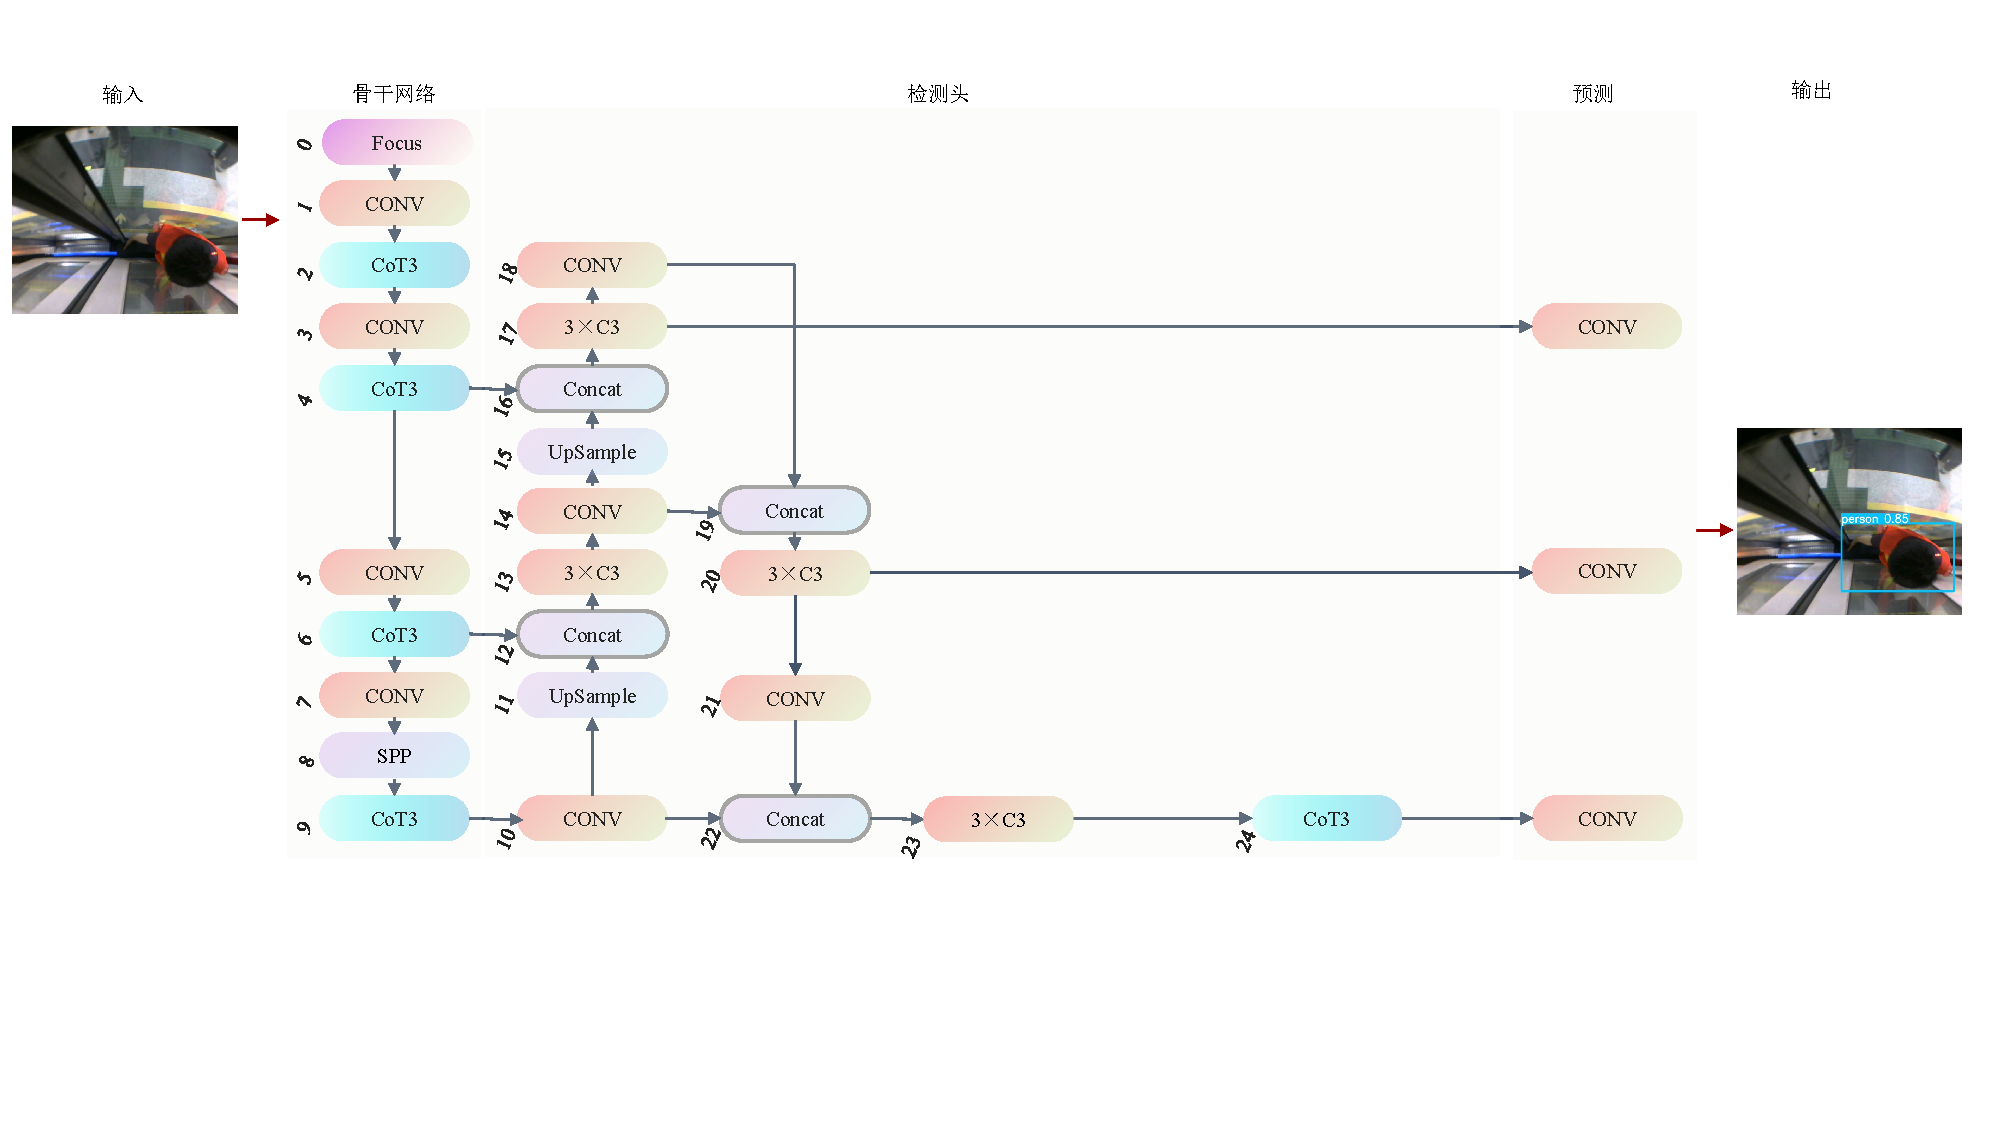
\includegraphics[scale=0.5]{Fig/GL-YOLO.pdf}
	\caption{\label{GL-YOLO}地铁屏蔽门与列车门间异物检测模型GL-YOLO结构}
\end{figure}

\subsection{基于K-Means++的锚框生成}
现有的锚框生成方法可以分为两类:手工方法和聚类方法。首先 anchor boxes 的尺寸是手工挑选的。虽然网络可以通过学习适当地调整 anchor boxes 形状,但是如果我们从一开始就为网络选择更好的 anchor boxes ,就可以让网络更容易学习并获得更好的检测结果。我们不用手工选择 anchor boxes,而是在训练集的边界框上的维度上运行 K-means 聚类算法,自动找到良好的 anchor boxes 。使用yolo系列通常需要通过kmeans聚类算法生成anchors,但kmeans算法本身具有一定的局限性,聚类结果容易受初始值选取影响。因此通过改进原kmeans\_for\_anchors.py实现 kmeans++聚类生成anchors。YOLOv5默认采用K-Means算法聚类COCO数据集生成的锚框,并采用遗传算法在训练过程中调整锚框,但是K-Means在聚类时,从其算法的原理可知,K-Means正式聚类之前首先需要完成的就是初始化个簇中心。同时,也正是因为这个原因,使得K-Means聚类算法存在着一个巨大的缺陷——收敛情况严重依赖于簇中心的初始化状况,采用K-Means++可以有效缓解这一问题,从而一定程度上能够提高检测精度和效果。K-Means++算法实际就是修改了K-Means算法的第一步操作之所以进行这样的优化,是为了让随机选取的中心点不再只是趋于局部最优解,而是让其尽可能的趋于全局最优解。要注意“尽可能”的三个字,即使是正常的K-Means++算法也无法保证百分百全局最优,在说取值原理之后我们就能知道为什么了思路就是我们要尽可能的保证各个簇的中心点的距离要尽可能的远当簇的中心尽可能的远的时候就能够尽可能的保证中心点之间不会在同一个簇内K-Means的迭代实际上就是簇的形状的修改,只要初始形状不太出格就会回归于正确形状。

\subsection{全局上下文信息与局部信息的结合}
如何较好的引入全局信息,而不造成太多计算量增加。以 VGGNet、Inception 系列和 ResNet 系列为代表的 2010-2020 年代的卷积神经网络 (ConvNets) 在多种视觉任务中取得了巨大的进展,它们的共同特点是顺序堆叠多个基本模块 (Basic Building Block),并采用金字塔结构 (pyramid network architecture),但是却忽略了显式建模全局上下文信息的重要性。SENet 模块系列模型突破了传统的 CNN 设计思路,将注意力机制引入到 CNN 中以捕获远程依赖,获得了更好的性能。

自从 2020 年以来,视觉 Transformer (ViTs) 进一步促进了视觉识别模型的发展,在 ImageNet 图像分类和下游任务上表现出比最先进的 ConvNets 更好的结果。这是因为与只进行局部建模的卷积操作相比,Transformer 中的自注意力机制能够对全局的成对依赖进行建模,提供了一种更有效的空间信息编码方法。然而,在处理高分辨率图像时,自注意力机制导致的计算成本是相当大的。许多研究表明,目标周围的背景信息对于提升目标检测的精度有着积极意义。而在地铁这一复杂巨系统中,上下文信息对于异物检测同样至关重要。然而,目前许多目标检测算法对于全局上下文信息的利用还不够充分:基于CNN的算法受限于感受野,缺乏全局建模的能力;而最近的基于Transformer的算法擅长于捕获长局依赖关系但是在局部特征采集上却力有未逮,因此限制了检测的精度。本章为了提升对异物的检测准确率,重点研究将全局上下文信息与局部信息相结合利用的目标检测方法。当前一些广泛使用的基于卷积神经网络的目标检测算法,如SSD[12]、YOLOv3-5[13-15]等在定位目标时仅使用候选目标区域内部的特征信息,而捕获全局上下文信息的能力不足。然而,一些研究[16-18]已经证实,全局上下文信息也可以为目标检测带来性能提升。例如,如果想要检测一张图片中的特定汽车,通常与目标同时出现的物体(比如人、道路或另1辆车)可能会为检测目标提供有用的线索。因此,全局上下文信息可以与局部信息相结合,为目标检测提供有用的指导。具体到地铁屏蔽门与列车门间异物检测这一任务,以图1来对使用全局上下文信息同局部信息相结合来进行异物检测这一过程进行说明:图1(a)中3个语义相关性更强的位置(1个真实的塑料袋及其2个倒影)拥有更高的置信度。同时,可能会影响模型检测性能的背景噪声被成功抑制。然后,将图1(a)中的全局上下文信息同图1(b)中的局部信息相结合,引导模型成功检测到异物(图1(c))。YOLOv5s在检测过程中只利用候选目标区域内部的特征进行检测。然而,对于整张图片来说,背景有时候也能够提供有用的信息。例如,如果想要检测1张图片中的特定汽车,通常与目标同时出现的物体(例如人、道路或另1辆车)可能会为检测目标提供有用的线索。当然,并不是所有的背景信息都有利于提高目标检测性能,一些无意义的背景噪声可能会损害检测性能。因此,如何有效的利用全局上下文信息是一个值得研究的问题。
大部分能够对全局上下文进行建模的注意力机制用于深度神经网络通常可以带来很好的性能提升,但将这些注意力机制应用于规模较小的网络中时,最终表现却不如将注意力机制应用于规模较大的深度神经网络。这主要是对于规模较小的网络来说,相比于引入注意力机制带来的效果提升,同时增加的大量运算是更无法接受的。以非局部[24]模块(如图4a)为例:非局部模块使用自注意力机制来对远程依赖进行建模。对于每个查询点,非局部模块首先计算查询点与所有点之间的成对关系以得到注意力图,然后通过加权和的方式聚合所有点的特征,从而得到与此查询点相关的全局特征,最终再分别将全局特征加到每个查询点的特征中,完成远程依赖的建模过程。非局部模块的这种操作,虽然有利于提升模型的检测效果,然而却导致了运算量过大的问题。同时,模型可以将这些全局上下文信息同局部特征信息相结合去检测异物,最终在提升模型检测效果的同时也不会大量增加模型的运算量。


\subsection{损失函数}

\section{实验与结果分析}
\subsection{实验数据集}
为了评估本章所提出算法GL-YOLO的性能,将在公开数据集PASCAL VOC及第三章所构建的FODD这两个数据集上同其他先进检测模型进行对比实验。
\subsubsection*{(1) PASCAL VOC}
PASCAL VOC\cite{pascalvoc07, pascalvoc12}是一个常用的分类、识别和检测视觉目标的基准数据集。它的特点是包含多样化的场景以及多种物体类别。PASCAL VOC提供了一整套从数据标注到算法评估的标准流程,它采用了一种名为xml的标注方法,数据集中的每一张图片对应一个xml格式的文件,其中包含了该图片的名称、图片尺寸、物体类型、位置、大小、是否完整和预测难度等信息。PASCAL VOC(2005-2012)竞赛的目标主要是进行图像目标检测,数据集中包含了生活中常见的20种物体,包括飞机、自行车、鸟、船、瓶子、公共汽车、小汽车、猫、椅子、奶牛、餐桌、狗、马、摩托车、人、盆栽、羊、沙发、火车和显示器。

PASCAL VOC有两个版本的数据集:VOC2007和VOC2012。VOC2007包含9963张标注过的图片,由train/val/test三部分组成,共标注出24,640个物体。而VOC2012是VOC2007数据集的升级版,一共有11530张图片。VOC2012的trainval/test包含08-11年的所有对应图片,并与VOC2007互斥,trainval中有11540张图片,共27450个物体。VOC2007和VOC2012数据集及二者的并集数据量对比如下表所示。
\begin{table}[htbp]
	\centering
	\small
	\caption{PASCAL VOC数据集详细信息}
	\setlength{\tabcolsep}{1.3mm}
	\begin{tabular}{ccccccccccc}
		\toprule[2pt]
		\multirow{2}[4]{*}{} & \multicolumn{2}{c}{训练集} & \multicolumn{2}{c}{验证集} & \multicolumn{2}{c}{训练与验证集} & \multicolumn{2}{c}{测试集} & \multicolumn{2}{c}{全部} \\
		\cmidrule{2-11}          & 图片数   & 目标数   & 图片数   & 目标数   & 图片数   & 目标数   & 图片数   & 目标数   & 图片数   & 目标数 \\
		\midrule
		VOC07 & 2501  & 6301  & 2510  & 6307  & 5011  & 12608 & 4952  & 12032 & 9963  & 24640 \\
		VOC12 & 5717  & 13609 & 5823  & 13841 & 11540 & 27450 & {\color{red} 11540} & {\color{red} 27450} & {\color{red} 23080} & {\color{red} 54900} \\
		总计    & 8218  & 19910 & 8333  & 20148 & 16551 & 40058 & {\color{red} 16492} & {\color{red} 39482} & {\color{red} 33043} & {\color{red} 79540} \\
		\bottomrule[2pt]
	\end{tabular}%
	\label{pascal voc}%
\end{table}%

表中,黑色字体所示数字是官方给定的,由于VOC2012数据集中测试集部分没有公布,因此红色字体所示数字为估计数据,按照PASCAL VOC通常的划分方法,即训练与验证集与测试集各占总数据量的一半。在后续的实验中,本章使用VOC2007的训练集+验证集和VOC2012的训练集+验证集训练,然后使用VOC2007的测试集测试,即在大多数论文中经常看到的07+12方法。
\subsubsection*{(2) FODD}

\subsection{评价指标}
在目标检测领域,均值平均精度(mean Average Precision, mAP)和每秒传输帧数(Frame Per Second, FPS)这两个评价指标是衡量目标检测算法准确性及检测速度的权威指标,被广泛应用于评价目标检测算法的性能。此外,由于本文所研究算法将面向实际应用,需要考虑到具体的硬件设备算力。因此,本文在此还将添加模型参数量(Parameters)、运算量(GFLOPs)作为额外的评价指标。下面给出这四个评价指标的具体计算方式:
\subsubsection*{(1) mAP}
\subsubsection*{(2) FPS}
\subsubsection*{(3) Parameters}
\subsubsection*{(4) GFLOPs}
\subsection{实验环境及超参数设置}
\subsection{FODD上的实验结果}
\subsection{PASCAL VOC上的实验结果}
\subsection{消融实验}

\section{本章小结}

	% 自行根据需要添加章节。

	\backmatter %章节不编号但页码继续
	%%%%%%%%%%%%%%%%%%%%%%%%%%%%%%%%%%%%%%%%%%%%%%%%%%%%%%%%%%%%%%    微调,使得后续章节的页眉不带章号——by MCH
	\renewcommand{\chaptermark}[1]{\markboth{#1}{}}
	%%%%%%%%%%%%%%%%%%%%%%%%%%%%%%%%%%%%%%%%%%%%%%%%%%%%%%%%%%%%%%
	\chapter{总结与展望}
\section*{主要研究内容}
\section*{未来展望} %结论
	 %%%%%%%%%%%%%%%%%%%%%%%%%%%%%%%%%%%%%%%%%%%%%% bibtex参考文献设置  (原版)
%%	\bibliographystyle{scutthesis}
%%	\bibliography{F:/MyLibrary}
	%%%%%%%%%%%%%%%%%%%%%%%%%%%%%%%%%%%%%%%%%%%%%%
	%%%%%%%%%%%%%%%%%%%%%%%%%%%%%%%%%%%%%%%%%%%%%% biber参考文献设置	——by MCH
	%\renewcommand*{\bibfont}{\refbodyfont}			% 设置文献著录字号比正文小一号(五号),需要小四号请注释该行. % 不推荐使用small,而是使用cls文件中精确定义了的字号。
	\phantomsection % “目录”中的链接能正确跳转,需要添加 \phantomsection 否则点击参考文献会跳转到结论
	\addcontentsline{toc}{chapter}{参考文献}	%目录中添加参考文献
	\printbibliography	% 参考文献著录
 	%%%%%%%%%%%%%%%%%%%%%%%%%%%%%%%%%%%%%%%%%%%%%%
 	% 只有一个附录
% 	\include{appendix}
 	% 有多个附录
	\include{appendix1} %附录1
	\include{appendix2} %附录2
 	%%%%%%%%%%%%%%%%%%%
	\chapter{攻读博士学位期间取得的研究成果} %博士/硕士记得选其一
\pubfont % 论文撰写规范里,这章是5号宋体,\pubfont 设置字号为5号了。但其实很多论文用小四号也OK。
一、已发表(包括已接受待发表)的论文,以及已投稿、或已成文打算投稿、或拟成文投稿的论文情况\underline{\textbf{(只填写与学位论文内容相关的部分):}}
\begin{table}
	\centering{}%
	\pubfont 
	\begin{longtable}{|>{\centering}m{0.5cm}|m{1.8cm}|>{\centering}m{2.8cm}|>{\centering}m{2.5cm}|>{\centering}m{2.2cm}|>{\centering}m{2.cm}|>{\centering}m{1cm}|}
		\hline 
		\textbf{序号} & \textbf{作者(全体作者,按顺序排列)} & \textbf{题 目} 						   & \textbf{发表或投稿刊物名称、级别} & \textbf{发表的卷期、年月、页码} & \textbf{与学位论文哪一部分(章、节)相关} &\textbf{被索引收录情况}\tabularnewline
		\hline 
		1    & 蒙超恒、裴海龙、程子欢					  & 涵道风扇式无人机的优先级控制分配 & 航空学报 & 已录用,2020年5月 & 2.1、2.2、3.4、4.1、4.2、5.1和5.3节 & EI\tabularnewline
		\hline 
		2	 & 	蒙超恒、裴海龙、程子欢						&  	Dynamic Control Allocation for A Twin Ducted Fan UAV							 & 2020 International Conference on Guidance, Navigation and Control  & 已录用,2020年8月 & 2.3、4.3和5.2节 &EI \tabularnewline
		\hline 
	\end{longtable}
\end{table}

注:在“发表的卷期、年月、页码”栏:

1.如果论文已发表,请填写发表的卷期、年月、页码;

2.如果论文已被接受,填写将要发表的卷期、年月;

3.以上都不是,请据实填写“已投稿”,“拟投稿”。

不够请另加页。

二、与学位内容相关的其它成果(包括专利、著作、获奖项目等)



%注:这部分一言难尽,我努力了很久都没有把这个表做好。感觉学校给的这个表的模板非常反人类。看国外大学的博士论文,那种像参考文献著录信息那样一行一行的,比较美观。而这个框框很难放文字进去。

\normalsize % \normalsize可以将下文调回和正文一样的字号,这个随个人喜好。注释掉的话,致谢就就跟随《攻读博士/硕士学位期间取得的研究成果》的字号。 %成果
	\chapter{致\texorpdfstring{\quad}{}谢}
%把下面文字替换
\begin{center}
这次你离开了没有像以前那样说再见,再见也他妈的只是再见 
~\\
我们之间从来没有想象的那么接近,只是两棵树的距离 
~\\
你是否还记得山阴路我八楼的房间,房间里唱歌的日日夜夜 
~\\
那么热的夏天你看着外面,看着你在消逝的容颜 
~\\
我多么想念你走在我身边的样子,想起来我的爱就不能停止 
~\\
南京的雨不停地下不停地下,就像你沉默的委屈 
~\\
一转眼,我们的城市又到了夏天,对面走来的人都眯着眼 
~\\
人们不敢说话不敢停下脚步,因为心动常常带来危险 
~\\
我多么想念你走在我身边的样子,想起来我的爱就不能停止 
~\\
南京的雨不停地下不停地下,有些人却注定要相遇 
~\\
你是一片光荣的叶子,落在我卑贱的心 
~\\
像往常一样我为自己生气并且歌唱 
~\\
那么乏力,爱也吹不动的叶子 
\end{center}
%把上面文字替换

~\\

\begin{minipage}[t]{0.945\textwidth}%
	\begin{flushright}
		戴愿\\
%		\today\\	% 自动时间
		2023年3月10日\\	%固定时间
		于华南理工大学
		\par\end{flushright}
\end{minipage}

 %致谢
\end{document}
